%%%%%%%%%%%%%%%%%%%%%%%%%%%%%%%%%%%%%
%Presentazione esame di Dottorato Davide Spataro
%presentation.tex
%Purpose: Main Beamer file for the presentation.
%@author Davide Spataro
%@version 1.0 14/01/2018 Eindhoven
%%%%%%%%%%%%%%%%%%%%%%%%%%%%%%%%%%%%

\documentclass{beamer}
\usetheme{Goettingen}

\AtBeginSection[]{
	\begin{frame}
	\vfill
	\centering
	\begin{beamercolorbox}[sep=8pt,center,shadow=true,rounded=true]{title}
		\usebeamerfont{title}\insertsectionhead\par%
	\end{beamercolorbox}
	\vfill
\end{frame}
}

\begin{document}
\title{Seamless Acceleration of numerical regular grid methods on manycore systems.}
\subtitle{Ph.D. in Mathematics and Computer Science\\ Universit\`a della Calabria}
\author{Davide Spataro} 
\date{January 19, 2018}

\frame{\titlepage} 


% Preamble
%%%%%%%%%%%%%%%%%%%%%%%%%%%%%%%%%%%%%
%Presentazione esame di Dottorato Davide Spataro
%preamble.tex
%Purpose: Contains a super short introduction plus information about me and the work I have done during these three years. 
% for each tests it shows graphs and table when available and also comment them.
%@author Davide Spataro
%@version 1.0 14/01/2018 Eindhoven
%%%%%%%%%%%%%%%%%%%%%%%%%%%%%%%%%%%%


%- Presentati, chi sei + Supervisors e la posizione che hai adesso
%- Posti in cui la tesi è stata sviluppata
%	- calabria + edimburgo + warwick
%	- fai in modo che si evincano le altre cose su cui hai lavorato
%	- velassco e il sistema lineari triangolari	
%

\section[Introduction]{Introduction}
\frame{\frametitle{Supervisors and Visiting Periods}
	\begin{center}
		\begin{block}{Supervisors}
				\begin{itemize}
					\item \textit{William Spataro}
					\item \textit{Donato D'Ambrosio}
				\end{itemize}
		\end{block}
		\pause
		\begin{block}{Visiting Periods}
			\begin{itemize}
				\item \textit{University of Edinburgh} (Scotland) - \textit{Prof. Jin Ooi} - \texttt{VELASSCO} EU project
				\pause
				\item \textit{University of Warwick} (England) - \textit{Prof. Gihan} Mudalige - \texttt{MPI+CUDA+SSE} Tridiagonal Systems  solver
			\end{itemize}
		\end{block}
	
		\pause
		\begin{block}{Current Position}
			\textit{Software Design Engineer}@\textit{ASML}, Metrology Department, Eindhoven, the Netherlands				
		\end{block}
	\end{center}
	

}

	\frame{\frametitle{Table of contents}\tableofcontents} 


% Introduction and Motivation
%%%%%%%%%%%%%%%%%%%%%%%%%%%%%%%%%%%%%
%Presentazione esame di Dottorato Davide Spataro
%introduction.tex
%Purpose: This file contains the introduction to the problem the thesis tries to solve, it shows why single chip performances are not improving as much as the moore's law predicts and introduces the concept of parallelism in computation and in numerical simulation.
%@author Davide Spataro
%@version 1.0 14/01/2018 Eindhoven
%%%%%%%%%%%%%%%%%%%%%%%%%%%%%%%%%%%%

%- La dimensione dei problemi che viene rislta oggigiorno è più grande. Il numero di applicazioni del calcolo scientifico sta aumentando con il numero di devices e di informazioni che la IoT sta fornendo. Questo implica che è richiesta una potenza di calcolo via via sempre maggiore
%
%- La potenza di calcolo aumentava fino a qualche anno fa in maniera esponenziale (mostra grafico) cioè raddoppiando il numero di transistor ogni anno. Ma questo trend non è più sostenibile per una serie di motivi (e ora che lavori in ASML te ne rendi ancora più conto). Dimensione dei transistor e calore per unita di superfice
%
%- Calcolo parallelo diventa fondamentale e negli ultimi 5 anni abbiamo visto un esplosione di parallelismo al punto che anche i telefoni sono macchine parallele con buone prestazioni. Fai esempio dei processori snapdragon.
%
%- Per cosa per esempio queste macchine nell'ambito del calcolo parallelo? risolvono equazioni differenziali etc. 
%Con che metodi lo fanno? molti, ma uno dei più usati è quello delle differenze finite. 
%
%Cosa fa questa tesi? 
 

\section{Motivations} 
\frame{\frametitle{Introduction and Motivations}
\centering
\begin{block}{}
	\centering 
\textbf{The amount of raw information available has increased dramatically during the last 10 years.}
\pause
	\begin{figure}
		\centering
			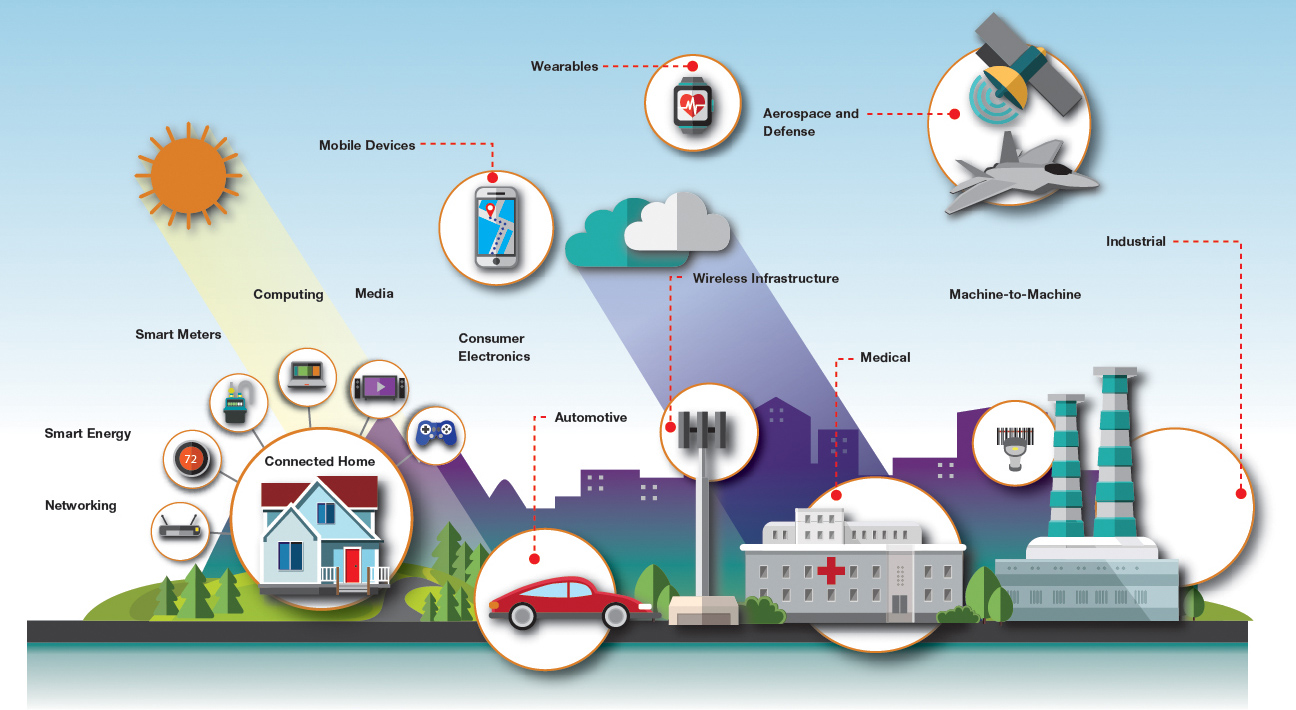
\includegraphics[scale=0.25]{images/broucer}
	\end{figure}
\end{block}
}

%%%%%%%%%%%%%%%%%%%%%%%%%%%%%%%%%%%%%%%%%%%

\frame{\frametitle{}
	\centering
	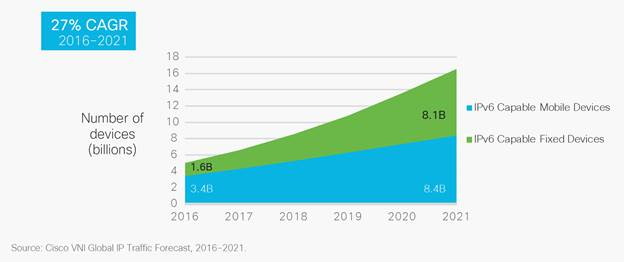
\includegraphics[width=8cm,height=4cm]{images/vni-hyperconnectivity-wp_7}
	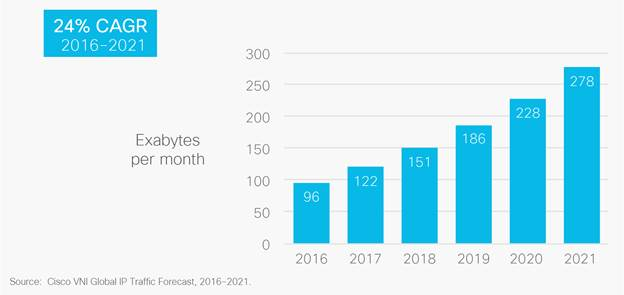
\includegraphics[width=8cm,height=4cm]{images/vni-hyperconnectivity-wp_0}
	
	
}

\frame{\frametitle{Need for Computational Power}
\begin{itemize}
	\item More data to process 
	\item Requirements for higher precision solvers
	
\end{itemize}
	\begin{figure}
	\centering
	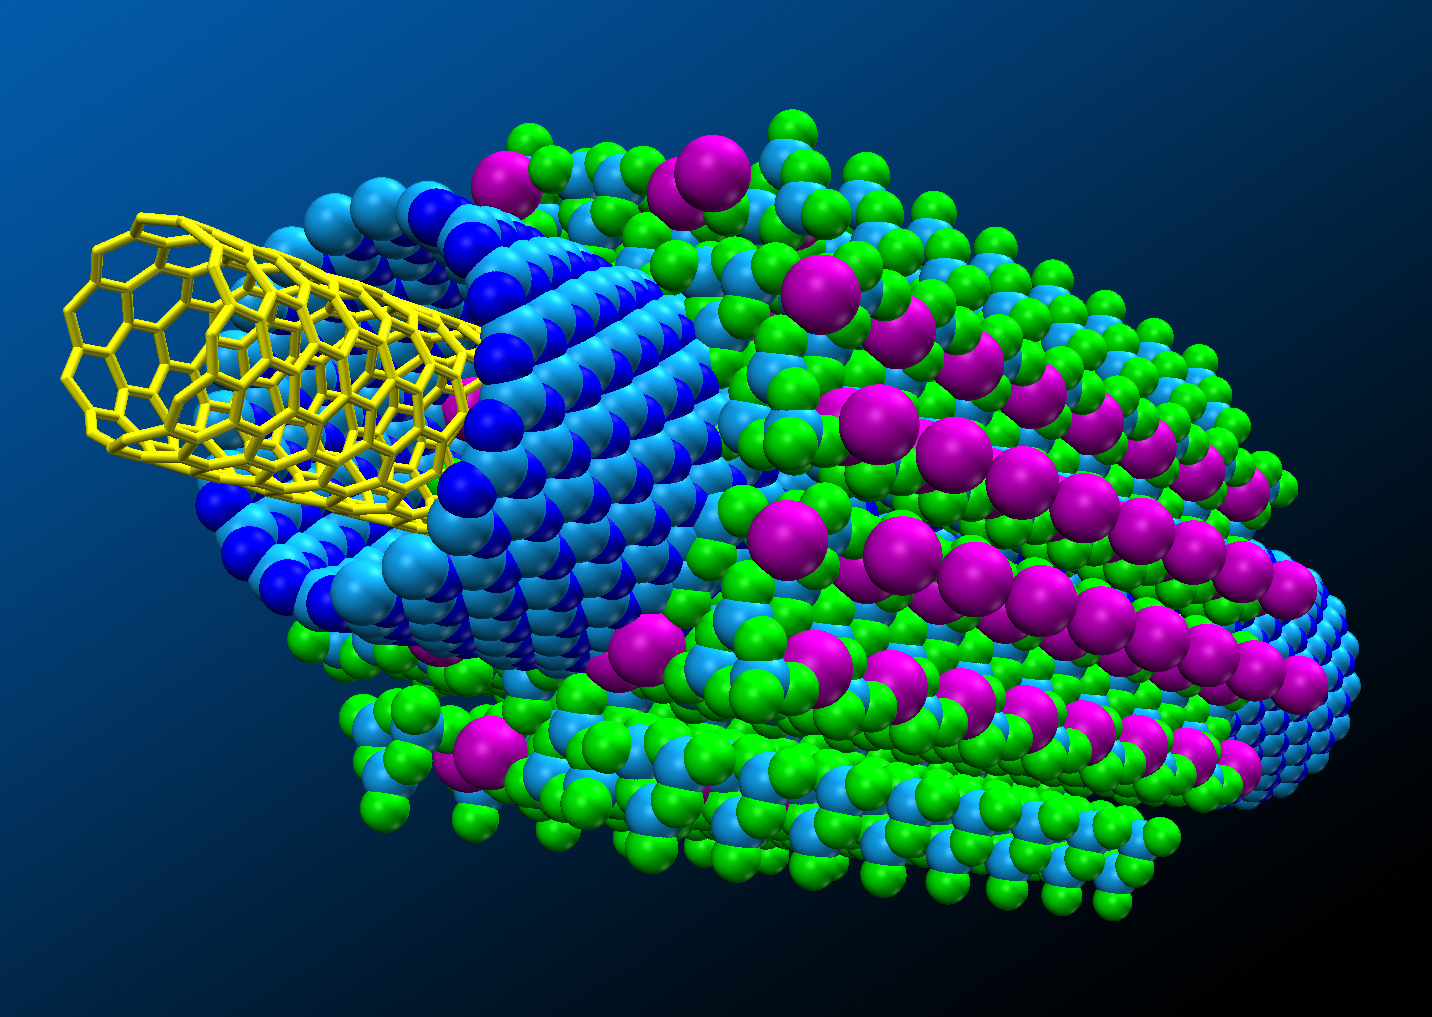
\includegraphics[width=0.8\textwidth]{images/material}
	\caption{Atomic Scale Simulation}
\end{figure}

}

%\frame{\frametitle{}
%	\centering
%	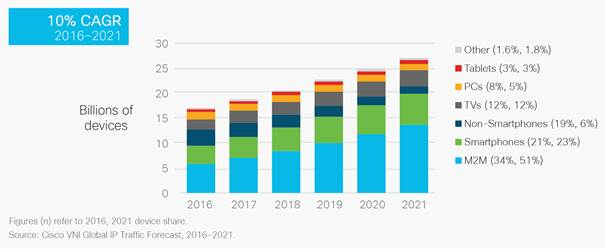
\includegraphics[width=8cm,height=4cm]{images/vni-hyperconnectivity-wp_2}
%	\pause
%	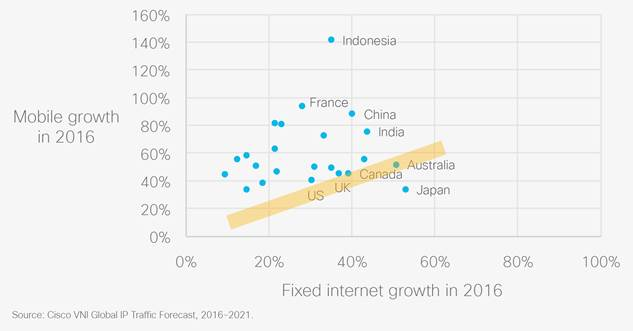
\includegraphics[width=8cm,height=4cm]{images/vni-hyperconnectivity-wp_1}
%}

\frame{\frametitle{Performance Improvements}
	\begin{center}
		\begin{block}{}
		 \begin{itemize}
		 	\item More Functional Units
		 	\item Higher Clock Speed
		 	\pause
		 	\item (A lot) More Transistor- Moore's Law
		 \end{itemize}
		\end{block}
	\end{center}
\begin{figure}
	\centering
	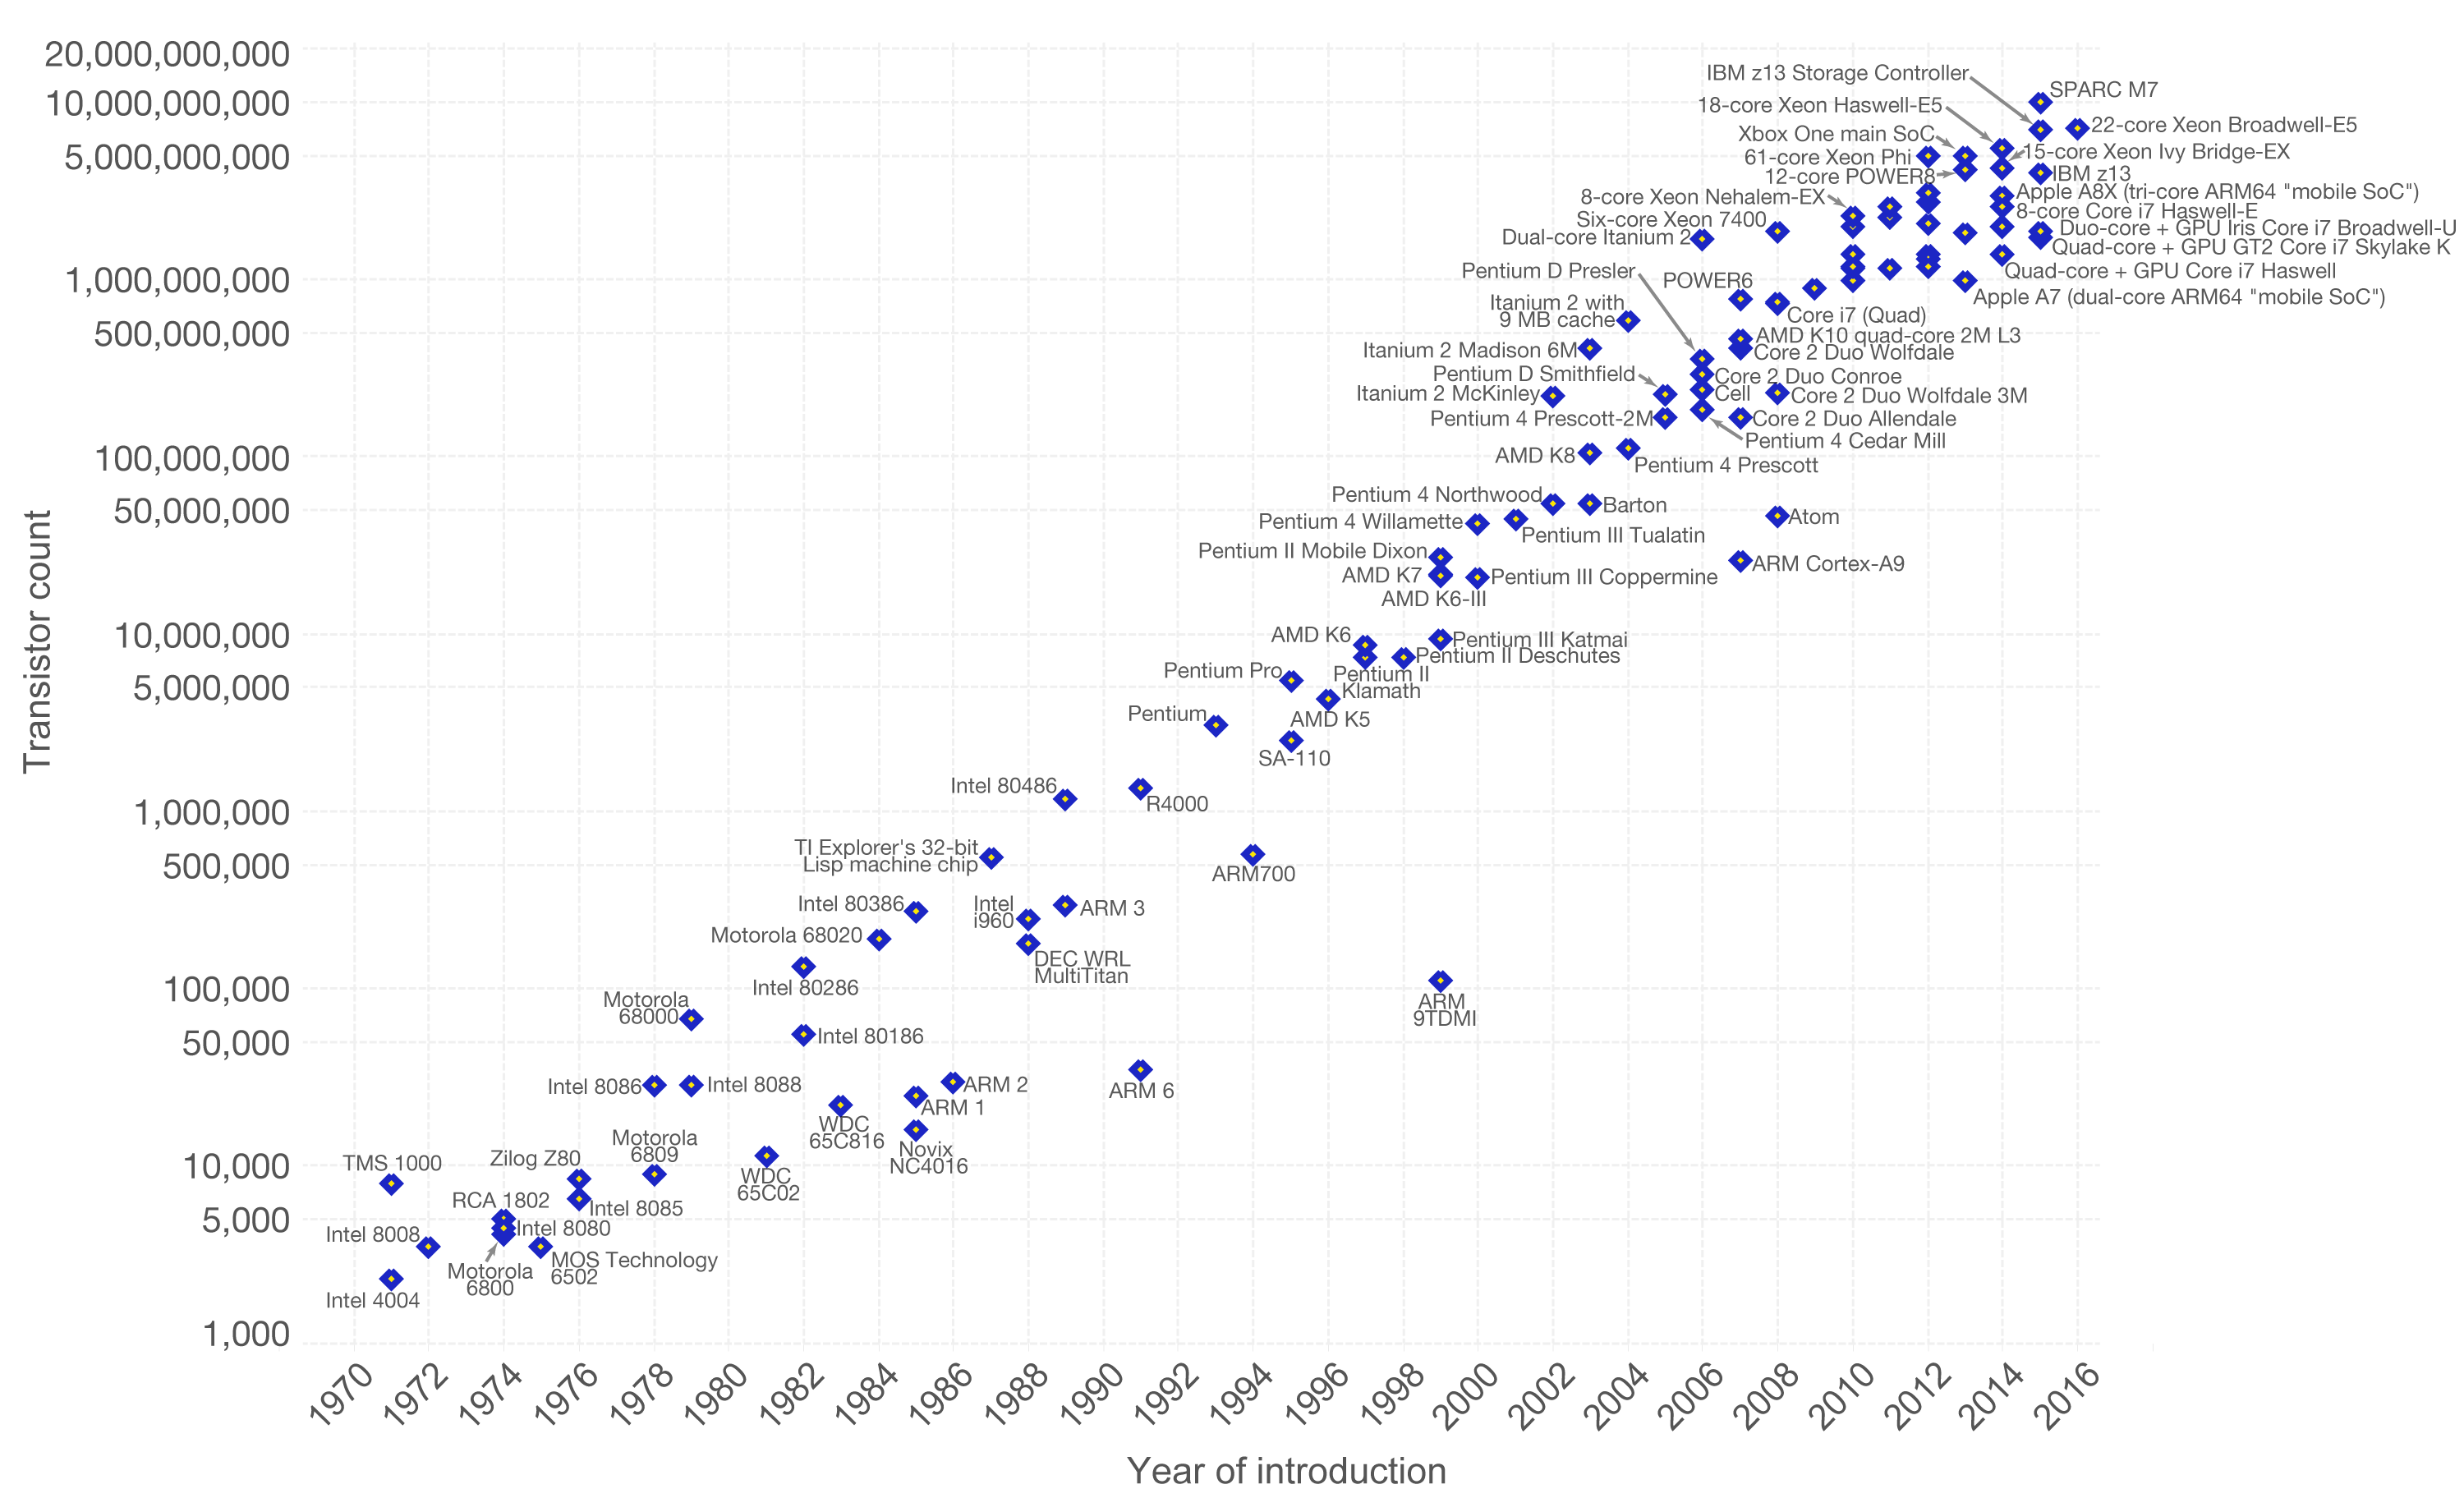
\includegraphics[width=0.8\textwidth]{images/moore_law2}
	\caption{Moore's law}
\end{figure}

}

%%%%%%%%%%%%%%%%%%%%%%%%%%%%%%%%%%%%%%%%%%%

\frame{\frametitle{This growth is not sustainable}
	\hfill \\
\centering
 Higher Clock and More Transistors = \textbf{More Heat}
 
\begin{figure}
	\centering
	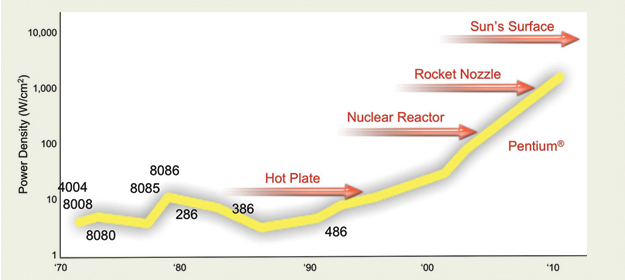
\includegraphics[width=\textwidth]{images/temperatureCPU}
\end{figure}
\pause
\begin{block}{Transistor size Limit} 
\begin{itemize}
	\item $7nm$ transistor is already possible
	\item $5nm$ will be in $4$ years
	\pause
	\item \textbf{Silicon atomic size is $0.2nm$!}
\end{itemize}	
\end{block}

}

\frame{\frametitle{Parallelism}
		\begin{itemize}
			\item Computational power demand is increasing
			\item Parallelism is the answer
			\item Almost every device has multiple computing core: phone, cars, laptop etc.
			\item Especially true for dedicated computing machine
		\end{itemize}	
	
	\begin{figure}
		\centering
		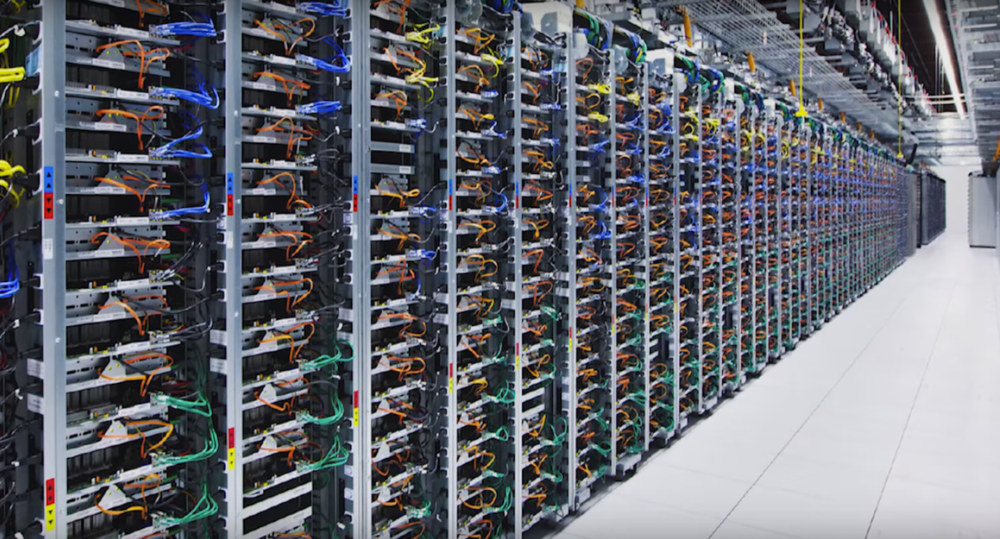
\includegraphics[width=\textwidth]{images/GoogleDataCenter}
	\end{figure}
}

\frame{\frametitle{Parallelism}
	\begin{block}{Trend in Scientific Computing HW}
		\begin{itemize}
			\item Large cluster of heterogeneous HW
			\item Heavy use of Accelerators (FPGA, Intel MIC, GPUs)
		\end{itemize}	
	\end{block}
\pause
\begin{block}{Programming heterogeneous HW}
	\begin{itemize}
		\item Is \textbf{very} complex
		\item Especially true for non parallel computing specialist
		\item One needs to master low-level details in order to write efficient solvers for such HW
	\end{itemize}	
\end{block}


}

\frame{\frametitle{Scope of the Thesis}
	\centering
	\textbf{The main goal of my work} 
	
\begin{itemize}
	\item a software framework for
	\item writing efficient solvers for regular grid methods
	\item targeting heterogeneous HW
\end{itemize} 
		\begin{figure}
		\centering
		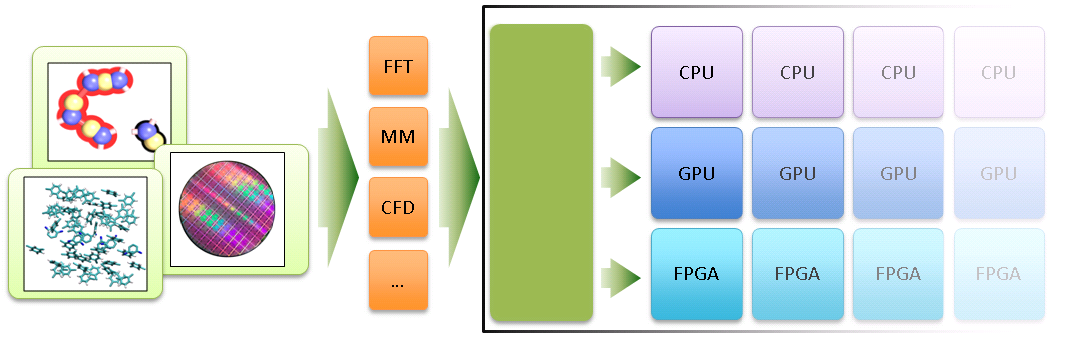
\includegraphics[width=\textwidth]{images/heterogen_modular_mapping}
	\end{figure}
}


%



%Introduction and Motivation
%%%%%%%%%%%%%%%%%%%%%%%%%%%%%%%%%%%%%
%Presentazione esame di Dottorato Davide Spataro
%numerical_methods.tex
%Purpose: This file contains a informal and formal description of the numerical methods that the content of this thesis addresses namely: Cellular Automata and Finite Difference Methods. 
%@author Davide Spataro
%@version 1.0 14/01/2018 Eindhoven
%%%%%%%%%%%%%%%%%%%%%%%%%%%%%%%%%%%%
\section{Numerical Simulation on Regular Grid} 
\frame{\frametitle{Motivation}
	
}
\subsection{Cellular Automata}
\frame{\frametitle{Cellular Automata}
	\begin{itemize}
		\item discrete $d$-dimensional lattice of sites
	\end{itemize}
	
}
\subsection{Finite Difference Method}
\frame{\frametitle{Finite Difference Methods}
	\begin{itemize}
		\item A DE is an equation where the unknown is a function
		\item e.g. Heat Equation: $\rho c\frac{\partial T}{\partial t} - \kappa \nabla^2T +Q=0$
		\item Boundary/Initial conditions are necessary e.g. temperature field at $t=0$
	\end{itemize}
\begin{figure}
	\centering
	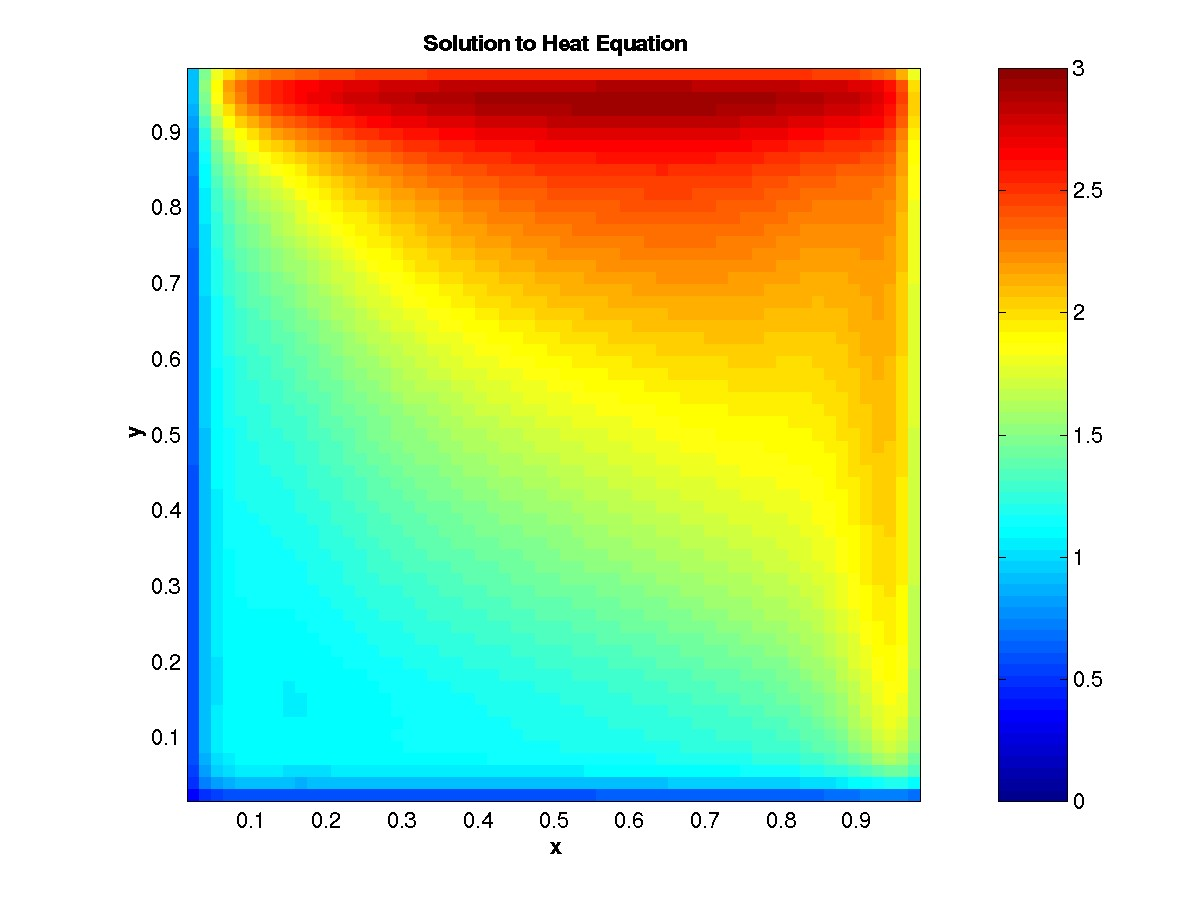
\includegraphics[width=0.8\textwidth]{images/heat2d_bc}
\end{figure}
	
}

\frame{\frametitle{Finite Difference Methods}
	\begin{itemize}
		\item Discovered by L. Euler and refined by Runge in 1910
		\item Differential operator is \textbf{approximated locally} using \textbf{finite number of values}
		\item Domain is partitioned in a grid-like fashion
		\item Solution is computed for the grid points only
	\end{itemize}
	\begin{figure}
		\centering
		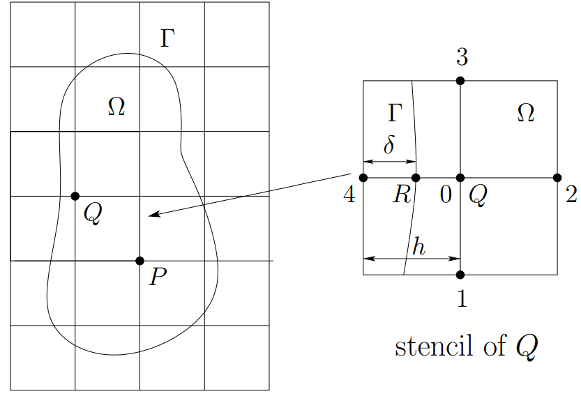
\includegraphics[width=0.8\textwidth]{images/gridcustom_shape2}
	\end{figure}
	
}

\frame{\frametitle{Finite Difference Formulas}
	\begin{itemize}
		\item Function approximating differential operator at a point using a finite number of neighbors
		\item Its arity determines the \textit{truncation order} of the formula
		\item The error is function of spacing between points in each direction 
		\item First order forward schema $\frac{\partial T(t,x)}{\partial x}  = \frac{T^n_{j+1} - T^n_{j}}{\Delta x} + \mathcal{O}(\Delta x)$ is obtained from: 
		 \[
		 T^n_{j+1} = T^n_{j} +
		\frac{\partial T}{\partial x}\bigg\rvert^n_j \Delta x +
		\frac{1}{2!}  \frac{\partial^2 T}{\partial x^2}\bigg\rvert_j \Delta x^2 + \ldots + 
		\frac{1}{k!}  \frac{\partial^k T}{\partial x^k}\bigg\rvert_j \Delta x^k + \ldots
		\]
		truncating at $k=1$ and solving for $\frac{\partial T}{\partial x}$

	\end{itemize}
}

\frame{\frametitle{Finite Difference Approximation of The Heat Equation}
	Given the initial value problem: $	\frac{\partial T(t,x)}{\partial t}=\kappa\frac{\partial^2 T(t,x)}{\partial x^2}$
\begin{itemize}
	\item Discretize the domain in a  1D regular uniform mesh
 	\item  first and second order derivative are substituted by forward and central difference formulas, respectively.
	\item Solving for $T^{n+1}_{j}$ leads to (explicit formula)
	\[
		 T^{n+1}_{j} = T^n_{j} + \frac{k \Delta t}{\Delta x^2} (T^n_{j+1}+T^n_{j-1}-2T^n_{j})
	\]
	\item The value for point at space coordinate $j$ at time $n+1$ can be obtained by using values of neighboring points i.e. $T^n_{j+1},T^n_{j-1},T^n_{j}$
\end{itemize}
}





%Opencal
\chapter[OpenCAL - The Open Computing Abstraction Layer]{The Open Computing Abstraction Layer for Extended
	Cellular Automata and the Finite Differences Method}
\label{ch:opencal}
\dictum[Gottfried Leibniz]{There are two kinds of truths: those of reasoning and those of fact. The truths of reasoning are necessary and their opposite is impossible; the truths of fact are contingent and their opposites are possible.}%
\vskip 1em

\lettrine[lines=3,lhang=0.33,lraise=0,loversize=0.15]{T}{his} chapter introduces \texttt{OpenCAL}, an open source computing
  abstraction layer defining a domain specific language for Extended
  Cellular Automata and the Finite Differences method (see chapters \ref{ch:CA} and \ref{ch:FDM} at page \pageref{ch:CA} and \pageref{ch:FDM} repectively). 
  Different implementations have been developed, which allow for transparent
  parallelism and are able to exploit multicore CPUs and manycore
  devices like GPUs, thanks to the adoption of \texttt{OpenMP} and OpenCL,
  respectively, as well as distributed memory architectures and/or multiple GPUs concurrently.
   System software architecture is presented and the
  underlying adopted data structures and algorithms are described in
  detail. Numerical correctness and efficiency have been assessed by
  considering the well known $SciddicaT$ Computational Fluid Dynamics
  landslide simulation model as reference example.  
  Moreover, a comprehensive study has been performed to device the best platform
  for execution as a function of numerical complexity and
  computational domain extent. Obtained results have highlighted the
  \texttt{OpenCAL} suitability for numerical models development and their execution on
  the most suitable high-performance parallel computational device.
  
\section{Introduction}
\label{sec:opencal_introduction}
 Scientific Computing \cite{golub2014scientific} is a broad and
  constantly growing multidisciplinary research field that uses formal
  paradigms to study complex problems and solve them through
  simulation by using advanced computing techniques and capabilities.
  
   Different formal paradigms have been proposed to provide the
  abstraction context in which problems are formalized. Partial
  Differential Equations (PDEs) were probably the first to be largely
  employed for describing a wide variety of phenomena. Unfortunately,
  PDEs can be analytically solved only for a small set of simplified
  problems \cite{Mazumder20161} and Numerical Methods have to be
  employed to obtain approximate solutions for real life applications. Among
  them, the Finite Differences Method (FDM) was one of the first
  considered, still currently employed, to address a wide variety of
  phenomena such as acoustics \cite{Chaigne19941112, Branski2014},
  heat \cite{Rana2012212, Sahin200619}, computational fluid dynamics
  (CFD) \cite{Chang1990317, Deng201390}, and quantum mechanics
  \cite{Hu2015640, Farrokhabadi201467} and many others.
  
  
  
Besides other solutions proposed for numerically approximating PDEs
  like, for instance, Finite Elements \cite{Hutton:2003} and Finite Volume Methods \cite{Moukalled}, further formal paradigms were more recently proposed for modeling complex systems. Among them, Cellular Automata (CA) \cite{vonNeumann:1966:TSA:1102024} are Turing-equivalent \cite{Codd:1968:CA:1098682, Cook04a} parallel computational models. CA are widely studied from a theoretical point
  of view \cite{Wolfram-1984, Langton-1990b, Wolfram-2002,
    Ninagawa201542}, and their application domains vary from
  Artificial Life \cite{Langton-1986, Beer2004309} to Computational
  Fluid Dynamics \cite{Frish&al-1986, McNamara&Zanetti-1988,
    Higuera&Jimenez-1989, Aidun2010439}, besides many others. See chapter \ref{ch:CA} for an extensive introduction on Cellular Automata.
    
Regardless from the adopted formal paradigm, the simulation of
complex systems often requires the execution of a very large number of computer instruction and this explains why nowadays scientific computing is very oftern linked to  Parallel Computing. 

\texttt{OpenMP} is the  most widely adopted solution for parallel programming on shared
  memory computers \cite{Chapman:2007:UOP:1370966}. It fully supports
  parallel execution on multi-core CPUs and, starting from the 4.0
  release, also includes support of accelerators like graphic
  processing units (GPUs) or Xeon Phi co-processors. Unfortunately,
  compiler support for the $4.0$ release is quite recent and, in
  practice, current \texttt{OpenMP} applications mainly run on CPUs
  \cite{Oliverio2011271, Amritkar2014501, pop:hal-00786675}. However,
  in recent years, general purpose computing on graphic processing
  units (GPGPU), which exploits GPUs and many-core coprocessors for
  general purpose computation, has gained wide acceptance as an
  alternative solution for high-performance computing, resulting in a
  rapid spread of applications in many scientific and engineering
  fields \cite{Owens200780}. Most implementations are currently based
  on NVIDIA CUDA (see e.g. \cite{Blecic2013, DAmbrosio2013630,
    DiGregorio20131183, DAmbrosio201230}), one of the first platforms
  proposed to exploit GPUs computational power on NVIDIA hardware. An
  open alternative to CUDA is OpenCL \cite{Stone201066}, an
  Application Program Inferface (API) originally proposed by Apple and
  currently managed by Khronos Group for parallel programming on
  heterogeneous devices like CPUs, GPUs, Digital Signal Processors
  (DSPs), and Field-Programmable Gate Arrays (FPGAs). Interest in
  OpenCL is continuously growing and many applications can already be
  found in literature \cite{Macri2015328, Bedorf20122825, Du2012391,
    Brown2011898}. However, an OpenCL parallelization of a scientific
  application is often a non-trivial task and, in many cases, requires
  a thorough refactorization of the source code. For this reason, many
  computational layers were proposed, which make many-core
  coprocessors computational power easier to be exploited. For
  instance, ArrayFire \cite{Malcolm2012} is a mathematical library for
  matrix-based computation such as linear algebra, reductions, and
  Fast Fourier transform; clSpMV \cite{Su2012353} is a sparse matrix
  vector multiplication library; clBlas \cite{clBlas-2016} is an
  OpenCL parallelization of the Blas linear algebra library. Examples
  of higher level computational layers, which provide the abstraction
  of formal computational paradigms, are OP2 \cite{Giles20131451},
  which is an open-source framework for the execution of unstructured
  grid applications on clusters of GPUs or multi-core CPUs, AQUAgpusph
  \cite{Cercos-Pita2015295}, which is a smoothed-particle
  hydrodynamics solver, and ASL \cite{asl}, an accelerated
  multiphysics simulation software based, among others, on the Lattice
  Boltzmann Method. Such high-level computational layers are briefly
  overviewed in the next section, together with some other significant
  examples.

This chapter is devoted to the description of \texttt{OpenCAL} which aims to be a portable parallel computing abstraction layer for scientific computing. \texttt{OpenCAL} is released under Lesser GNU Public Licence (LGPL) version 3 and is freely downloadable from GitHub at the following link: \url{https://github.com/OpenCALTeam/opencal}. \texttt{OpenCAL} allows for  the definition of computational models based on CA, XCA and FDM. It is designed to be easily extended and applied to all computational methods based on regular and uniform grids. 
The implementation descripted in this chapter targets shared multicore, distributed memory and GPUs and is designed to make the parallelism transparent to the user addressing and hiding many aspects of the underlying formal computational model and parallel execution platform. 

%\subsection{An Overview on Scientific Simulation Software}
%In this section, we present a non-exhaustive overview of some
%  interesting and widely adopted parallel computing simulation software, which provide a high-level approach for the modeling of complex systems, hiding  low-level implementation issues such as memory allocation/de-allocation, thread management, and I/O  operations.General purpose simulation software,
%  like Mathematica or Matlab, are intentionally not considered here.
%\subsubsection{DEVS}
%  DEVS \cite{Zeigler:1997:DEH:615253.615512, Zeigler:2000:TMS:580780},
%  abbreviation of Discrete Event System Specification, is a modular
%  and hierarchical formalism for modeling and analyzing general
%  systems which can be described in terms of state transition
%  tables. It also allows to describe continuous state systems (which
%  can be formalized in terms of differential equations), and hybrid-
%  continuous state and discrete event systems. The basic DEVS
%  formalism allows to describe the inputs, outputs and states of a
%  model (called atomic), besides the relationships among
%  them. Furthermore, atomics can be used as building blocks for larger
%  coupled models. Both atomic and coupled models adopt the same
%  interface protocol, allowing to use a model as a component in
%  another, larger model. Several extensions to the original DEVS
%  formalism have been developed. Among these, P-DEVS
%  \cite{Chow:1994:PDP:193201.194336} is a modeling formalism which
%  provides both conceptual and parallel execution benefits with
%  respect to the original DEVS formalism, while Cell-DEVS
%  \cite{Wainer:2009:DMS:1611320} is an extension of the DEVS formalism
%  that allows the definition of Cellular Automata models. A wide
%  variety of models have been developed using this approach, such as
%  fire spreading models with different conditions, formation of a
%  watershed and robots in a manufacturing plant
%  \cite{Troccoli:2001:MCP:882496.884491}.
%\subsubsection{OP2}
%  OP2 \cite{Giles20131451} is an open-source framework for the
%  execution of unstructured grid applications on clusters of GPUs or
%  multi-core CPUs. The main characteristic of the library is the use
%  of source-to-source translation to generate efficient back-end code
%  for state-of-the-art hardware for the different target
%  platforms. Specifically, OP2 aims to separate the scientific
%  specification of an application from its parallel implementation to
%  achieve code endurance and near-optimal performance by re-targeting
%  the back-end to different multi-core/many-core hardware. The OP2
%  \emph{active} library approach uses program transformation tools, so
%  that a single application code written using the OP2 API is
%  transformed into the appropriate form that can be linked against a
%  target parallel implementation (e.g. OpenMP, CUDA, OpenCL, MPI,
%  etc.) enabling execution on different back-end hardware
%  platforms. In order to facilitate the development of unstructured
%  mesh applications at a higher hardware agnostic level, OP2 provides
%  both a C/C++ and a Fortran API. This enables application developers
%  to focus on solving problems at a higher level and not worry about
%  architecture specific optimisations. As a consequence, the problem
%  domain space can be separated into both a higher application level
%  to concentrate on solving domain specific problems and write code
%  that remains unchanged for different underlying hardware, and in the
%  meanwhile consider a lower implementation level, that focuses on how
%  a computation can be executed most efficiently on a given platform
%  by carefully analysing the data access patterns.  The performance
%  impact of the library design choices have been quantified on a range
%  of NVIDIA GPUs using the end-to-end performance of an industrial
%  representative CFD application (Airfoil) developed using the OP2
%  API. The full OP2 source, the Airfoil test case code and the
%  auto-tuning framework are available as open source software
%  \cite{OP2Web}.
%\subsubsection{CAMELot}
%  CAMELot \cite{dattilo2003simulation, Mendicino2006, d2007parallel}
%  is a proprietary CA and XCA high performance simulation environment
%  derived from CAMEL \cite{cannataro1995parallel}. The system supports
%  CARPET, a purpose-built language for CA programming based on C with
%  additional constructs to describe the rule of the state transition
%  function of a single cell of a cellular automaton and, eventually, to steer the
%  application. Specifically, a CARPET program is composed of a declaration part that
%  describes the properties of CA (dimension, radius, state, neighbour,
%  parameters, region), a body program that implements the transition
%  function, and a steering part that contains a set of commands for
%  extracting and analysing system information and performing
%  computational steering (i.e., global operations). The steering
%  section is performed by the runtime system at each iteration, after
%  the transition functions of all cells have been evaluated.  The
%  state of a cell is defined as a record of typed \emph{substates}
%  (char, shorts, integers, floats, doubles and one-dimensional
%  arrays), and even complex neighbourhoods (e.g., hexagonal, Margolus)
%  can be simply defined by means of a CARPET
%  statement. Non-deterministic, time-dependent and non-uniform
%  transition functions can also be defined. Camelot offers an
%  integrated programming environment, an interactive user interface
%  and permits the efficient and seamless simulation of XCA on
%  distributed memory computers.
%\subsubsection{libAuToti}
%  An open-source alternative to CAMELot is libAuToti
%  \cite{spingola2008modeling}, an efficient and flexible parallel XCA
%  library. Similarly to CAMELot, libAuToti allows for a simple and
%  concise definition of both the transition function and the other
%  characteristics of XCA model definition. It allows for both
%  sequential and parallel execution, both on shared and distributed
%  memory machines (thanks to the adoption of the Message Passing
%  paradigm for the interprocesses communications), by hiding parallel
%  implementation issues to the user. The library also implements a
%  dynamic load balancing algorithm to better exploit computational
%  resources and reduce overall execution time
%  \cite{DBLP:conf/csc/ZitoDSSRA09}. A multithread version was also
%  developed to better exploit multi-core architectures, coupled with
%  an interactive 2D/3D visualization system based on VTK
%  \cite{spataro2010multithread}.
%\subsubsection{ASL}
%  The Advanced Simulation Library (ASL) \cite{asl} is a free and open
%  source hardware accelerated multiphysics simulation software. It is
%  based, among others, on the Lattice Boltzmann Method and is written
%  in OpenCL, which enable efficient deployment on a variety of
%  massively parallel architectures. However, no OpenCL knowledge is
%  strictly required to develop ASL-based applications, thanks to a
%  simplified C++ API. ASL can be used to model various coupled
%  physical and chemical phenomena and employed in a multitude of
%  fields like computational fluid dynamics, computer-aided
%  engineering, and crystallography.  Mesh-free, immersed boundary
%  approach allows to move from CAD directly to computations
%  eliminating pre-processing efforts and reducing amount of potential
%  errors.
%\subsubsection{AQUAgpusph}
%  Eventually, AQUAgpusph \cite{CercosPita2015295} is a free Smoothed
%  Particle Hydrodynamics (SPH - a mesh-free Lagrangian method to solve
%  Navier-Stokes equations) software accelerated with OpenCL. The main
%  advantages with respect to other existing SPH libraries are the use
%  of OpenCL instead of CUDA, which allows for parallel execution on a
%  variety of massively parallel devices, the implementation of the
%  most popular boundary conditions, the easy customization of the code
%  to different problems, the extensibility with regard to Python
%  scripts and the runtime output which allows the tracking of
%  simulations in real time, or a higher frequency in saving some
%  results without a significant performance lost. Authors have proven
%  to improve the solver speed, the results quality, and the usability
%  for a wider areas of application.
  
\section[Software Architecture]{\texttt{OpenCAL} Software Architecture and the Considered Parallel Computing Paradigms}
  This section describes the software architecture of the first
  \texttt{OpenCAL} release. As described in Figure \ref{fig:architecture}, a
  computational model can be designed at the higher level of
  abstraction. As already stated, supported computational paradigms
  are CA, XCA and FDM. At this level, the main features of the
  computational model like dimensions, neighborhood, boundary
  conditions, involved substates and elementary processes, are
  designed. The simulation process, which allows to obtain the model
  evolution at discrete time steps, is also defined at this level, by
  specifying the initial condition of the system, global operations
  (like steering or global reductions), the initial and final
  computational step and a possible stopping criterion. Eventually,
  optimizations can be considered, namely the explicit update, which
  allows to selectively update substates after the application of each
  elementary process, and the quantization feature, which allows to
  restrict the computation to a subset of the computational domain, by
  excluding stationary cells.
  
  \begin{figure}
  	\begin{center}
    \includegraphics[width=1.0\textwidth]{./images/opencal/Figure05}
    \caption{\texttt{OpenCAL} architecture. At the higher level of abstraction, the models,
    	as well as the simulation process, and possible optimizations are
    	designed. \texttt{OpenCAL} can be found at the implementation abstraction
    	layer, allowing for a straightforward implementation of the designed
    	model. In fact, it can be considered as a domain-specific language for
    	the CA, XCA and FDM computational methods, built on top of the C
    	language and the \texttt{OpenMP} and OpenCL APIs. \texttt{OpenCAL} applications can be
    	executed at the hardware level on both multi-core CPUs and many-core
    	devices, while the execution on cluster is planned but currently not
    	supported.}
    \label{fig:architecture}
  \end{center}
\end{figure}
  
   \texttt{OpenCAL} can be found in the implementation abstraction level. As it
  can be seen, four different versions can be considered for
  implementing the previously designed computational model, namely
  \texttt{OpenCAL}, \texttt{OpenCAL-OMP} and \texttt{OpenCAL-CL} and \texttt{OpenCAL-MPI}. The first one refers to the   serial implementation of the library, while second and the third are \texttt{OpenMP}  and OpenCL-based parallelizations, respectively, as pointed out by
  the language/low-level library level. The fourth one is a cluster ready implementation that allows to execution on distributed memory cluster where each node can exploit multiple GPUs.
  All implementations are written in C for the maximum efficiency and provide high-level data types and functions that match the XCA formal components, allowing  for a straightforward implementation of the designed computational
  model, by also allowing to ignore low-level issues like memory
  management and I/O operations. In this respect, \texttt{OpenCAL} can be
  considered as a domain-specific language (DSL) for the CA, XCA and
  FDM computational methods. Finally, at the hardware level, depending
  on the adopted version of the library, execution can be performed on
  single- and multi-core CPUs, or on many-core accelerators like GPUs,
  almost transparently to the user.
  
   Figure \ref{fig:architecture} also shows hybrid MPI+Open-MP and
  MPI+OpenCL parallel implementations of \texttt{OpenCAL}, which will allows to
  exploit clusters of CPUs and many-core accelerators. 

  Note that an \texttt{OpenMP}-based parallelization is generally more
  straightforward with respect to one based on OpenCL or MPI and, when
  compilers will fully support the 4.0/4.5 \texttt{OpenMP} specifications, it
  will be possible to execute \texttt{OpenMP}-based applications on both
  multi-core CPUs and many-core high-performance devices. On the other
  hand, an OpenCL-based parallelization allows to exploit a wide range
  of high-performance many-core devices straight away and, with greater control on the underlying hardware and on the execution flow, allowing better exploitation of the hardware capabilities. 
 For these reasons, both the \texttt{OpenMP} and OpenCL versions of \texttt{OpenCAL} have been developed and are maintained. 
  
\section{The Open Computing Abstraction Layer}
\label{sec:OpenCAL}
In this section we describe the API of the serial version of
\texttt{OpenCAL}, which allows for the definition of 2D and 3D CA, XCA and
FDM models, and their execution on CPUs. Nevertheless, 1D models can
also be defined as degenerate case of 2D ones. The implementation of
a simple 2D CA, namely the \textit{Conway's Game of Life}
\cite{gardner1970a}, is shown in this section as first and
straightforward example of application.

\subsection{API naming Convention}
In \texttt{OpenCAL}, besides the three basic supported scalar data types,
namely \verb'CALbyte', \verb'CALint', and \verb'CALreal', which
redefine the \verb'char', \verb'int' and \verb'double' C native
scalar data types, respectively, the API adopts the following
conventions:
\begin{itemize}
	\item Derived data types are characterised by the \verb'CAL' prefix,
	followed by a type identifier formed by one or more capitalised
	keywords, an optional suffix identifying the model dimension
	(\verb'2D' or \verb'3D'), and an eventual optional suffix
	specifying the basic scalar type (\verb'b', \verb'i', or \verb'r',
	for \verb'CALbyte', \verb'CALint' and \verb'CALreal' derived
	types, respectivey);
	\item Constants and enumerals are characterised by the \verb'CAL_'
	prefix, followed by one or more uppercase keywords separated by
	the \verb'_' character (e.g. the \verb'CAL_TRUE' and
	\verb'CAL_FALSE' boolean-type values);
	\item Functions are characterised by the \verb'cal' prefix, followed
	by at least one capitalized keyword, and end with a suffix
	specifying the model dimension (\verb'2D' or \verb'3D') and the
	basic datatype (\verb'b', \verb'i', or \verb'r', for
	\verb'CALbyte', \verb'CALint' and \verb'CALreal' derived types,
	respectively).
\end{itemize}
Moreover, the \verb'{arg1|arg2|...|argn}' and
\verb'[arg1|arg2|...|argn]' conventions are adopted in the
following. The first one identifies a list of $n$ mutually exclusive
arguments, where one of the arguments is needed, while the second a
list of $n$ non-mutually exclusive optional arguments.

Among derived data types, \verb'CALParameter{b|i|r}' represents an
alias for the corresponding basic \texttt{OpenCAL} scalar data type, and can
be optionally used for defining model parameters.


\subsection{API}
An \texttt{OpenCAL} model is declared as a pointer to \verb'CALModel{2D|3D}'
and defined by means of the \verb'calCADef{2D|3D}()' function. The
model object stores the dimensions of the computational domain in
terms of number of rows and columns (and also slices in case of a 3D
model), the computational domain boundary topology (e.g., if a 2D
computational domain has to be considered as a bounded or an
unbounded torus), the neighbourhood pattern, and also registers
pointers to substates and elementary processes composing the
transition function. Moreover, it manages a sub-structure which
allows to exploit the built-in quantization feature by means of
which, based on user-specified criteria, the computation can be
restricted to a subset of non-stationary cells (also called active
cells) of the whole computational domain.

 As regards neighborhoods, \texttt{OpenCAL} provides a set of predefined
patterns. For instance, the \verb'CAL_MOORE_NEIGHBORHOOD_{2D|3D}'
enumeral refers to the Moore pattern (cf. Figures
\ref{fig:2Dneighborhood}b and \ref{fig:3Dneighborhood}b). von
Neumann 2D and 3D neighborhoods are also predefined, as well as 2D
hexagonal patterns (cf. Figures \ref{fig:2Dneighborhood}c and
\ref{fig:2Dneighborhood}d). Custom neighborhoods can also be defined
in \texttt{OpenCAL} by considering the \verb'CAL_CUSTOM_NEIGHBORHOOD_{2D|3D}'
enumeral and the \verb'calAddNeighbor{2D|3D}()' function, which adds
a cell to the neighbourhood by means of its relative coordinates
with respect to the central one. Note that, a zero-based index is
assigned to the neigbouring cells in order to address them without
the need to provide their relative coordinates, as shown in Figures
\ref{fig:2Dneighborhood} and \ref{fig:3Dneighborhood}.
\begin{figure}[!htbp]
	\begin{center}
		\includegraphics[width=1.0\textwidth]{./images/opencal/Figure01}
		\caption{Examples of von Neumann (a) and Moore (b) neighborhoods for two-
			dimensional CA with square cells. Examples of Moore neighborhoods are also shown for hexagonal CA, both for the cases of horizontal (c) and vertical (d) orientations. Central cell is represented in dark gray, while adjacent cells are in light gray. A reference system is here considered to evaluate cells coordinates in terms of row and column indices in a matrix-style representation, and a 0-based numerical identifier assigned to each cell in the neighborhood for straightforward access}
		\label{fig:2Dneighborhood}
	\end{center}
\end{figure}
Elementary processes, both local interactions and internal
transformations, are defined by means of callback functions and
registered to a computational model by means of the
\verb'calAddElementaryProcess{2D|3D}()' function. Each elementary
process callback must return \verb'void' and takes a list of integer
arguments, representing the coordinates of a generic cell in the
computational domain. Elementary processes define the \texttt{OpenCAL}
transition function, and can be implicitly applied by the simulation
loop to the cells of the computational domain in the same order in
which they were registered to the computational model, or in a user
defined order (cf. below).


\begin{figure}[!htbp]
	\begin{center}
		\includegraphics[width=1.0\textwidth]{./images/opencal/Figure04}
		\caption{Examples of von Neumann (a) and Moore (b, b') neighborhoods for
			three-dimensional CA with cubic cells. Central cell is represented in
			dark gray, while adjacent cells are in light gray. A reference system
			is here considered to evaluate cells coordinates in terms of row,
			column and slice indices in a matrix-style representation, and a
			0-based numerical identifier assigned to each cell in the neighborhood
			for straightforward access.}
		\label{fig:3Dneighborhood}
	\end{center}
\end{figure}
Substates are defined as pointers to
\verb'CALSubstate{2D|3D}{b|i|r}' and can be registered by means of
the \verb'calAddSubstate{2D|3D}{b|i|r}()' function. Substates are
internally defined by means of two linearized arrays (also called
computational layers), having the same dimensions of the
computational domain. The \emph{current} layer is used as a
read-only memory for retrieving central and neighboring cells
current states, while the \emph{next} one for updating the new value
for the central cell. This is a commonly adopted solution for
obtaining the \emph{implicit parallelism}, thanks to which cells
appear to be simultaneously updated with respect to each other, even
in the case of serial computation. Single layer substates can be
also defined in \texttt{OpenCAL} by simply registering them through the
\verb'calAddSingleLayerSubstate{2D|3D}{b|i|r}()' function. In this
case, they only consist of the current computational layer, and can
be used for internal transformations processing. To retrieve the
current value of a substate for a (central) cell by providing its
coordinates within the computational domain, the
\verb'calGet{2D|3D}()' function can be adopted, while the
\verb'calGetX{2D|3D}()' function can be considered for obtaining the
same information for a neighbouring cell, by providing an additional
parameter specifying the index of the cell in the neighborhood
(cf. Figures \ref{fig:2Dneighborhood} and \ref{fig:3Dneighborhood}
for predefined neighborhoods). Eventually, the
\verb'calSet{2D|3D}()' function can be used to set the new value of
a substate for the (central) cell to the next computational
layer. In the case of a single layer substate, the
\verb'calSetCurrent{2D|3D}{b|i|r}()' function has to be employed for
updating purposes. It acts like the \verb'calSet{2D|3D}()' function,
with the exception that the new value is written on the current
computational layer. Note that, after the application of each
elementary process, all the registered substates are implicitly
updated, i.e. the next layer is copied into the current
one. However, this behaviour can be overridden and substates
explicitly, as well as selectively, updated by means of the
\verb'calUpdateSubstate{2D|3D}{b|i|r}' function
(cf. below). Obviously, single layer substates do not need to be
updated.

The \texttt{OpenCAL} quantization feature is implemented by considering a
dynamic array of active cells, $A$, which is initially empty. An
array of flags, $F$, having the same dimension of the computational
domain is also considered, which is initially set to
\verb'CAL_FALSE' in each position. Eventually, an integer variable,
$size$, initially set to zero, is used to evaluate the new dimension
of $A$ per effect of the add/remove operations. In order to add a
cell to $A$, the \verb'calAddActiveCell{2D|3D}()' function can be
used, which sets the flag value to \verb'CAL_TRUE' in the
corresponding position of the array $F$ and increases $size$ by
one. Similarly, the \verb'calAddActiveCellX{2D|3D}()' function adds
a neighbouring cell to $A$. Eventually, the
\verb'calRemoveActiveCell{2D|3D}()' function can be used to remove a
cell from $A$, by contextually modifying the corresponding flag in
$F$ and decrementing $size$ by one. When an add/remove stage is
completed, e.g. after the execution of an elementary process, and
the (scattered) array $F$ is well defined, the set $A$ must be
updated. The update process deletes the current set $A$, allocates a
new set of active cells of dimension $size$, and applies a
straightforward serial stream compaction algorithm by processing the
entire array of flags $F$, as shown in Figure
\ref{fig:active_cells}. As evident, the algorithm has a $O(n)$
computational efficiency, being $n$ the number of cells of the
cellular space $R$. In this way, only the loop updating $A$ occurs
on the whole computational domain (since the $F$ array must be fully
checked). In fact, when $A$ is not empty, it is processed instead of
the whole computational domain and both elementary processes
computation and substates updating take place on the active
cells. As substates, even $A$ is implicitly updated at the end of
each elementary process. However, active cells update can also be
explicitly performed by means of the
\verb'calUpdateActiveCells{2D|3D}' function (cf. below).
Eventually, note that the add and remove stages updating the values
in $F$ have to be performed separately, e.g. by two different
elementary processes. In fact, if the same elementary process could
both add and remove cells depending for instance on the current
state of the central cell, two different cells could update the same
(neighbouring) cell to different activation states, and the
resulting value in $F$ would depend on the (serial) application
order of the elementary process, giving rise to a possible logical
error.

\begin{figure}
	\begin{center}
		\includegraphics[width=1.0\textwidth]{./images/opencal/Figure06}
		\caption{An example of application of the serial stream compaction algorithm
			adopted to update the set $A$ of active cells in the serial
			implementation of \texttt{OpenCAL}. In the example, active cells are
			represented in gray within a two-dimensional 4x4 matrix of flags,
			implemented as a linearized array, $F$. The stream compaction
			algorithm simply processes $F$ and produces the compacted array $A$ as
			output, containing the coordinates of the active cells. The global
			state transition is therefore limited to the cell in $A$, and a new
			configuration of the system obtained. The process is therefore
			repeated at the next computational step.}
		\label{fig:active_cells}
	\end{center}
\end{figure}

In order to perform a simulation, a pointer to \verb'CALRun{2D|3D}'
must be declared and defined by means of the
\verb'calRunDef{2D|3D}()' function. The simulation object stores a
pointer to the \texttt{OpenCAL} model to be run, a step counter, the initial
and final computational steps, an enumeral of type
\verb'CALUpdateMode', which specifies the substates update policy
(if implicit or explicit), and registers a set of four optional
callback functions. These latter, described below, take a pointer to
an \texttt{OpenCAL} model as argument and do not return any value, with the
exception of the termination function, which returns a
\verb'CALbyte' (\verb'CAL_TRUE' if the termination criterion is
satisfied, \verb'CAL_FALSE' in the other case). The optional
callback functions are:
\begin{itemize}
	\item \verb'init()': It can be used to set the initial conditions of
	an \texttt{OpenCAL} computational model. It can be registered to the
	simulation object by using the \verb'calRunAddInitFunc{2D|3D}()'
	function. If defined, the \verb'init()' function is executed once
	before the simulation loop.
	\item \verb'globalTransition()': It can be used to redefine the
	execution order of the registered elementary processes and to
	perform selective substate updating. The
	\verb'calApplyElementaryProcess{2D|3D}()' function can be used
	within the registered callback to apply a registered elementary
	process to each cell of the computational domain, while the
	\verb'calUpdateSubstate{2D|3D}{b|i|r}' to update a registered
	substate. The \verb'globalTransition()' function also allows to
	call functions that can perform global operations over the
	computational domain, e.g. reductions. It can be registered to the
	simulation object by using the
	\verb'calRunAddGlobalTransitionFunc{2D|3D}()' function. If
	defined, the \verb'globalTransition()' function overrides, i.e. is
	applied instead of, the implicit global transition function.
	\item \verb'steering()': It can be used to perform global
	operations, e.g. reductions, at the end of each computational
	step, that is after that all the elementary processes have been
	applied. Predefined reductions allow to compute global minimum,
	maximum, sum, product, as well as logical and bit-wise AND, OR and
	NOT operations on the registered substates. A steering can be
	registered to the simulation object by using the
	\verb'calRunAddSteeringFunc{2D|3D}()' function. If defined, the
	\verb'steering()' function is applied at the end of each
	computational step.
	\item \verb'stopCondition()': It can be used to define a stopping
	criterion for the simulation. Note that, if the last computational
	step was set to \verb'CAL_RUN_LOOP', the \verb'stopCondition()'
	callback is mandatory to stop the simulation. It returns
	\verb'CAL_TRUE' if the termination criterion is satisfied,
	\verb'CAL_FALSE' in the other case. The termination callback can
	be registered by using the
	\verb'calRunAddStopConditionFunc{2D|3D}()' function. If defined,
	the \verb'stopCondition()' function is executed at the end of each
	computational step.
\end{itemize}
The simulation process can be executed by means of the
\verb'calRun{2D|3D}' function. Algorithm \ref{algo:simuloop}
outlines the \texttt{OpenCAL} implicit simulation process, which takes place
in the case the enumeral \verb'CAL_UPDATE_IMPLICIT' was used as last
argument for the \verb'calRunDef{2D|3D}()' function. The
\verb'init()' function, if defined, is called first and then active
cells (if quantization is enabled) and substates are
updated. Moreover, the \verb'step' counter and the \verb'halt'
variable, that is used to check the simulation termination
condition, are set to the initial step and to \verb'CAL_FALSE',
respectively. The main simulation loop follows, which applies
elementary processes in the order they were registered to each cell
of the computational domain. After the execution of each elementary
process, active cells and substates are updated. If defined, the
\verb'steering()' global function is therefore called and active
cells and substates updated. The \verb'stopCondition()' function is
also called and the step counter increased. The simulation loop
continues while the \verb'halt' variable, whose value is set by the
\verb'stopCondition()' function, is \verb'CAL_FALSE' or the final
step of computation is met.

\begin{algorithm}
	\DontPrintSemicolon \SetKwFunction{Init}{init()}
	\SetKwFunction{Update}{update}
	\SetKwFunction{Steering}{steering()}
	\SetKwFunction{Stop}{stopCondition()}
	\SetKwFunction{Finalize}{finalize()}
	
	\Init \tcp*{Call the \Init global function}
	 \If{quantization}{
		\Update($A$) \tcp*{Update the array of active cells}
	 }
	\ForAll{$q \in Q$}
		{ \Update($q$) \tcp*{Update the substate $q$}
		}
	$step \gets initial\_step$\; $halt \gets false$\;
	\While{$\neg$halt $\land$ (step $\leq$ final\_step $\vee$
		final\_step = CAL\_RUN\_LOOP)}{
		 \ForAll{$e$ of $\sigma$}{
			\ForAll{$(A \neq \emptyset \land i \in A) \vee$ $i \in R$}
				{
				$e(i)$ \tcp*{Apply the elementary process $e$ to the cell
					$i$}
				}
			\If{quantization}{
				 \Update($A$) \tcp*{Update the array of active cells} 
			}
			\ForAll{$q \in Q$}{ 
				\Update($q$) \tcp*{Update the substate $q$}
			 }
		  }
	  	\Steering \tcp*{Call the \Steering global function}
	  	 \If{quantization}{
	  	 	 \Update($A$) \tcp*{Update the array of active cells}
  	 	  } 
   	  	\ForAll{$q \in Q$}{
			\Update($q$) \tcp*{Update the substate $q$}
		 }
		 $halt \gets $\Stop \tcp*{Check the stop condition} $step \gets step + 1$\;
	 }
	\Return\;
	\caption{{\texttt{OpenCAL} main implicit simulation process.}}
	\label{algo:simuloop}
\end{algorithm}

Explicit update can be set by using the \verb'CAL_UPDATE_EXPLICIT' enumeral as last argument of the \verb'calRunDef{2D|3D}()' function. In this case, the global transition function must be overridden and both active cells and substates explicitly updated. Eventually, instead of the \verb'calRun{2D|3D}()', which executes the whole simulation process, the
\verb'calRunCAStep{2D|3D}()' function can be used to apply a single
step of the global transition function, including steering and stop
condition checking. In this case, the initialization function must
be called explicitly, as well as the simulation counter increased.




\subsection{\texttt{OpenCAL} Conway's Game of Life}
As a first illustrative example, we here present the \texttt{OpenCAL}
implementation of the Turing complete Conway's Game of Life\cite{gardner1970a}, one of the most simple, yet powerful examples of CA, devised by mathematician John Horton Conway in 1970. See Section \ref{sect:GOL} at page \pageref{sect:GOL} for a formal definition of \textit{The Game of Life} and a  description of its governing rules.

The program in Listing \ref{lst:cal_life} provides a complete
\texttt{OpenCAL} implementation of Game of Life in just few lines of code,
by defining both the CA model and the simulation object, needed to
let the CA evolve step by step.

%%%% GOL listing C serial implementation %%%%
    \lstset{language=[OpenCL]C,
	caption=An \texttt{OpenCAL} implementation of the Conway's Game of
	Life., 
	label=lst:cal_life, 
	basicstyle=\footnotesize\ttfamily,
	keywordstyle=\color{blue}\ttfamily,
	stringstyle=\color{red}\ttfamily,
	commentstyle=\color{green}\ttfamily,
	backgroundcolor=\color{light-gray}, 
	numbers=left, 
	numberstyle=\tiny
}
\lstinputlisting{./code/cal_life.c}
%%%%%%%%%%%%%%%%%%%%%%%%%%%%%%%%%%%%%%%%%%%%
\texttt{OpenCAL} header files are included at lines 1-3. Specifically,
\verb'cal2D.h' allows to define 2D CA and substates,
\verb'cal2DRun.h' the simulation object, while \verb'cal2DIO.h'
provides some basic I/O functions. The CA object is declared at
line 6, while lines 7 and 8 declare a substate and a simulation
object, respectively.  Objects declared at lines 6-8 are defined
later in the \verb'main' function. In particular, the \verb'life'
CA object is defined at line 24 by the \verb'calCADef2D()'
function. The first 2 parameters define the dimensions of the
computational domain (in terms of number of rows and columns,
respectively), while the third the Moore
neighborhood. Furthermore, the fourth parameter sets a toroidal
topology for the cellular space, while the last switches the
active cells optimization to off.

The CA simulation object is defined at line 25 by the
\verb'calRunDef2D()' function, where the first parameter is a
pointer to the \verb'life' CA object, while the second and third
parameters specify the initial and last simulation steps,
respectively. Eventually, the last parameter sets the update
policy to implicit.

Line 27 allocates memory and registers the integer-based $Q$
substate to the CA by means of the \verb'calAddSubstate2Di()'
function, while line 29 registers an elementary process by means
of the \verb'calAddElementaryProcess2D()' function. Here, the
\verb'lifeTransitionFunction' parameter represents the name of a
developer-defined function implementing the transition function
rules (cf. lines 10-20). Within the elementary process, the
\verb'calGet[X]2Di()' and \verb'calSet2Di()' functions are used
for reading and updating purposes, respectively. The
\verb'calInitSubstate2Di()' function at line 31 sets the whole $Q$
substate to the value 0 (for both the current and next
layers). Lines 32-36 define a so called \emph{glider} pattern
(cf. Figure \ref{fig:cal_life_glut}a) by means of the
\verb'calInit2Di()' function. The \verb'calSaveSubstate2Di()'
function at line 38 saves the $Q$ substate to file, while the
\verb'calRun2D()' function at line 40 enters the simulation
process (actually, only one computational step in this example),
and returns to the \verb'main' function when the simulation is
terminated. The \verb'calSaveSubstate2Di()' is called again at
line 42 to save the new (last) configuration of the CA, while the
last two functions at lines 44 and 45 release memory previously
automatically allocated by \texttt{OpenCAL} for the CA, substates
(actually, only $Q$ in this case) and simulation object. The
\verb'return' statement at line 47 ends the program.

Figure \ref{fig:cal_life_glut} show a graphical representation of
the initial and final configurations of Game of Life,
respectively, as implemented in Listing \ref{lst:cal_life}. As
expected, the glider initially defined has evolved into the new
correct configuration.

\begin{figure}
	\begin{center}
		\includegraphics[width=1.0\textwidth]{./images/opencal/Figure07.pdf}
		\caption{An \texttt{OpenGL/GLUT} version of the Game of Life, as implemented in Listing \ref{lst:cal_life}, showing the (a) initial and (b) final configurations of the system. Alive cells are represented in white, dead cells in blue.}
		\label{fig:cal_life_glut}
	\end{center}
\end{figure}

\section{The \texttt{OpenCAL} \texttt{OpenMP}-based Parallel Implementation}
\label{sec:OpenCAL-OMP}

In this section we present \texttt{OpenCAL-OMP}, the \texttt{OpenMP}-based parallel
implementation of \texttt{OpenCAL}, which allows for seamless parallel execution on
shared memory computing systems in a SIMD fashion. For brevity, we
only present and discuss differences with respect to \texttt{OpenCAL} in
terms of API and internal algorithms.
Since one of the main goal is to obtain transparent parallelism, the \texttt{OpenCAL-OMP} API has been designed to differ as less as possible to the serial
one, leading to the adoption of the same naming conventions, interface,
and programming model.

Double layer substates were also considered in \texttt{OpenCAL-OMP}, which permitted a straightforward lock-free \texttt{OpenMP} parallelization. In fact no race conditions can occur, since the current layer is accessed in read mode, and the update phase access to the next layer is limited to the memory location associated with
the central cell. As a consequence, elementary processes and
substates updating loops, as well as global reduction operations,
were parallelized by simply considering lock-free \texttt{OpenMP} pool of
threads, as shown in Figure \ref{fig:pool_of_threads}. In the
example, a pool of three threads were used to partition the
computational domain in three subregions, which were therefore
processed in parallel both during the application of an elementary
process and the subsequent substates updating. Note that, in the
case only a subset of cells are actually involved in computation, as
in the example, load unbalance conditions can occur. In fact, the
third thread is wasted, since it only applies the elementary process
on a subset of stationary cells. A dynamic \texttt{OpenMP} scheduling is
adopted in this case to mitigate the unbalance among chunks.
\begin{figure}
	\begin{center}
		\includegraphics[width=1.0\textwidth]{./images/opencal/Figure08.pdf}
		\caption{An example of \texttt{OpenCAL-OMP} parallel application of an elementary
			process to a substate $Q$ and its subsequent parallel updating. The
			computational domain is initially partitioned by means of a pool of
			three threads (fork phase). These latter concurrently apply the
			elementary process by reading state values from the current layer and by updating new values to the next one. At the end of the elementary process application, threads implicitly synchronize by joining into the master one (join phase), and the parallel update phase starts. As before, a pool of threads concurrently copies the next layer into the current one and the new configuration of $Q$ is obtained. A join phase eventually occurs, which ensures data consistency before the application of another elementary process.}
		\label{fig:pool_of_threads}
	\end{center}
\end{figure}
As regards the quantization feature, it is still based on the
dynamic array of active cells $A$, containing the coordinates of non
stationary cells, and on the array of flags $F$, having the same
dimension of the computational domain, used to register the cells
activation state during the application of the transition
function. $F$ is initially set to \verb'CAL_FALSE' in each position
and, each time a cell has to be added to/removed from $A$, the
corresponding position in $F$ is updated by a \verb'CAL_TRUE'/\verb'CAL_FALSE' value. 
At the end of the add/remove
stage, a lock-free parallel stream compaction is executed on the
resulting scattered array $F$ to obtain the new set of active cells
$A$. For this purpose, $F$ is partitioned over the $N$ running
threads. Each of them builds a private subset, $A_p$ $(p=0, 1,
\ldots N-1)$, of cells to be added to/removed from $A$, by
contextually evaluating its relative size, $size_p$. Eventually, the
actual $size$ of $A$ is obtained as $size = \sum_{p=0}^{N-1}
size_p$, and the subsets $A_p$ assembled together to form the new
set $A$, as shown in Figure \ref{fig:active_cells_omp}. As for the
case of the \texttt{OpenCAL} serial stream compaction, it is evident that
also in this case the algorithm has a $O(n)$ computational
efficiency, where $n$ is the number of cells of the cellular
space. Note that, being both the \verb'CAL_TRUE' and \verb'CAL_FASE'
8-bit long enumerals, no inconsistent values can be obtained even in
the case more than one thread accesses the same location in $F$
simultaneously and, therefore, a lock-free updating policy was also
here considered for the quantization optimization. However, as for
\texttt{OpenCAL}, the add and remove stages updating the values in $F$ have
to be performed separately, e.g. by two different elementary
processes, in order to avoid possible race conditions. In fact, if
the same elementary process could both add and remove cells
(depending for instance on the current state of the central cell),
two different threads applying the elementary process to two
different cells could update the same (neighbouring) cell to
different activation states. In this case, the resulting value in
$F$ would depend on which thread writes the value for last, giving
rise to a possible logical error. Eventually, note that the
quantization feature is able to optimally distribute the
computational load over the running threads, since stationary cells
are simply excluded by the computation (cf. Figure
\ref{fig:active_cells_omp}). A more efficient static \texttt{OpenMP}
scheduling is therefore here adopted instead of the dynamic one.

\begin{figure}
	\begin{center}
		\includegraphics[width=1.0\textwidth]{./images/opencal/Figure09}
		\caption{An example of application of the parallel stream compaction algorithm used in \texttt{OpenCAL-OMP} to update the set $A$ of active cells. Active cells are represented in gray within a two-dimensional 4x4 matrix of flags, implemented as a linearized array, $F$. The parallel stream
			compaction algorithm processes $F$ by means of a lock-free pool of
			threads, resulting in the $A_p$ $(p=0,1,2)$ partial arrays of active
			cells. These latter are eventually assembled together by the master
			thread, resulting in the compacted array $A$. A new pool of threads
			therefore applies the state transition function in parallel on $A$
			with an optimal load balancing, and a new configuration of the system
			is obtained. The process is therefore repeated at the next
			computational step.}
		\label{fig:active_cells_omp}
	\end{center}
\end{figure}


\subsection{\texttt{OpenCAL-OMP} implementation of the Game of Life}
Conway's Game of Life can be straightforwardly implemented in
parallel by using \texttt{OpenCAL-OMP}. The source code is almost identical
to the one in Listing \ref{lst:cal_life}, with the exception of
the first three lines, where the \texttt{OpenCAL-OMP} header files are
included instead of the OpenCAL ones. For this purpose, it is
sufficient to change the headers parent directory from
\verb'OpenCAL' to \verb'OpenCAL-OMP'. For instance, the
\verb'OpenCAL/cal2D.h' header is replaced by
\verb'OpenCAL-OMP/cal2D.h'. The remaining lines of code are
unchanged and therefore source code is omitted. As for the case of
the \texttt{OpenCAL} implementation, Figure \ref{fig:cal_life_glut} shows
the initial and final configuration of the system.


\section{The \texttt{OpenCAL} OpenCL-based Parallel Implementation}
\label{sec:OpenCAL-CL}
  In this section, we present the OpenCL-based parallel implementation
of OpenCAL, which allows for the parallel execution on both shared
memory computing systems and many-core acceleration devices in a
SIMD fashion, by highlighting the differences with respect to the
serial and OpenMP implementations of OpenCAL in terms of API and
internal algorithms.

The API is very similar to the serial one and adopts the same
programming model and naming conventions, with the exception that
the \verb'calcl', \verb'CALCL' and \verb'CALCL_' prefixes are
adopted for functions, data types and constants, respectively. The
main difference with respect to OpenCAL and OpenCAL-OMP is that an
OpenCAL-CL application is subdivided in two parts, one running on
the CPU, the other in parallel on a compliant device. The host
application defines the host-side computational model, registers the
required substates to it, while elementary processes and other
global function are implemented as OpenCL kernels and registered to
a device-side computational model. When a device-side model is
defined, data registered to the host-side model is implicitly copied
to the compliant device global memory, transparently to the
user. Within kernels, however, the user can transfer data to the
local memory and then update the global memory when the local
operations are complete, for better performance. Data stored in
global memory is therefore copied back to the host at the end of
the simulation process. This latter if equivalent to that of OpenCAL
and OpenCAL-OMP (cf. Algorithm \ref{algo:simuloop}), with the
exception that kernels are executed device-side and the simulation
process can not be currently, in this first OpenCAL release, made explicit.

Grid of work-items can be two- or three-dimensional, depending on
the dimension of computational model, if 2D or 3D, respectively. In
the case the quantization feature is exploited, a one-dimensional
grid is considered. The number of work-items is evaluated for each
model dimension by preliminary querying OpenCL for the
(device-dependent) preferred work-group size multiple (i.e. the
warp/wavefront size in NVIDIA/AMD GPUs), $w_s$, and therefore by
considering the smallest multiple of $w_s$ which is greater than or
equal to the model dimension. For instance, if $w_s=32$ and the
first dimension of the domain is 2000, the number of work-items in
that dimension will be 2016, i.e. the first multiple of 32 which is
greater than or equal to 2000, thus resulting in 16 redundant
work-items. However, since redundant work-items do not map any cell
of the computational domain, they immediately terminate their
execution. Moreover, according to OpenCL, work-items are grouped in
workgroups. The choice of the number of workgroups to be considered,
and therefore the workgroup size, depends on the device architecture
and is automatically determined by default, transparently to the
user. These choices should allow to not waste resources and also
permits the user to ignore low-level hardware details. In any case,
the \verb'calclSetWorkGroupDimensions{2D|3D}()' function can be used
to explicitly set the workgroup size.

Double layer substates are also considered in OpenCAL-CL. That is,
as for the serial and OpenMP-based versions of OpenCAL, the current
layer is used for reading the states of the neighboring cells, while
the next for updating the new value for the central one. A grid of
OpenCL work-items can therefore be defined, each one executing the
transition function on a different cell of the computational domain,
independently to each other. In fact, no race conditions can occur,
since access to the current layer is read-only, and each work-item
updates a different memory location of the next layer. Being the
data stored in global memory, work-items can be easily synchronized
after the execution of each elementary process, since a global
barrier is implicitly defined at the end of each kernel
execution. The kernel-based transition function is therefore applied
by considering the one-thread/one-cell parallel execution policy
and, at the end of each computational step, substates are updated
device side, avoiding the need to perform time consuming data
transfer between host and device.

The quantization feature is also supported in OpenCAL-CL, where
coordinates of the active cells are stored in the array $A$ that,
differently from the serial and OpenMP-based implementations, is
static and has the same dimension of the computational domain. A
variable, $size$, initially set to zero, is also considered to
identify the actual number of active cells. A static array of flags,
$F$, is also considered, which has the same dimension of the
computational domain. It is initially set to \verb'CAL_FALSE' in
each position, to mark all cells as inactive. The add/remove
operations, performed by work-items at the init stage or during the
execution of the transition function, update the array of flags $F$
as in the previous discussed implementations. In case of concurrent
access to the same location of $F$, data integrity is guarantied
only under the condition work-items execute the same instruction
(e.g. all of them write the \verb'CAL_TRUE' value). In fact, if the
same instruction is executed by more than one work-item (even
belonging to different workgroups) to the same location in global
memory where $F$ is stored, the access is serialized and at least
one access is guarantied (even if which actual thread performs the
operation is undefined - cf. e.g. \cite{CUDA}). Moreover, the same
considerations discussed for the OpenCAL and OpenCAL-OMP
implementations of the active cells optimization, even hold for the
OpenCAL-CL one. As a consequence, to both guaranty data integrity
and to avoid possible logical errors, the add and remove stages have
to be performed separately, e.g. by two different elementary
processes. At the end of each add or remove stage, cells to be
considered active are marked by the \verb'CAL_TRUE' value in the
scattered array $F$. In order to update $A$, a parallel stream
compaction algorithm is considered. $F$ is partitioned in $N$
chunks, being $N$ the number of considered work-items, and the
following three stages applied:
\begin{enumerate}
	\item Each work-item counts the number of active cells in its chunk
	of the array $F$. As a result, an array $S$ is obtained, where
	$s_p$ ($p = 0, 1, \ldots, N-1$) is the number of the active cells
	counted by the $p^{th}$ work-item;
	\item A prefix-sum algorithm is executed to both evaluate the total
	number of active cells, $size$, and a further array, $O$, where
	$o_p$ ($p = 0, 1, \ldots, N-1$) represents the offset to be
	considered by the $p^{th}$ work-item from which it must start
	entering in $A$ the coordinates of the cells that are marked as
	active in its chunk of the array $F$.
	\item Each work-item processes its chunk of $F$ and enters in $A$
	the coordinates of the cells marked as active, starting from the
	offset $o_p$ ($p = 0, 1, \ldots, N-1$) computed in the previous
	stage.
\end{enumerate}
For illustrative purposes, the above three stages are graphically
represented in Figure \ref{fig:streamcompaction}. At step $t$, the
configuration of the cells actually involved in the computation are
represented in gray in a two-dimensional 4x4 matrix, corresponding
to the linearized scattered array $F$. The parallel stream
compaction algorithm processes the scattered array $F$ to obtain the
compacted array $A$, containing the coordinates of the three active
cells in its first three positions. A two-block grid with two
threads per block is considered in the example, which adopt the one
thread/one active cell execution policy. Note that, at step $t$ a
total of four work-items are considered to process a set of three
active cells. In this case, the thread that does not match any
active cell immediately terminates. Among the parallel stream
compaction stages, the prefix-sum algorithm at stage two, which
evaluates the array $O$ of offsets, is crucial for the overall
efficiency of the algorithm. 
\begin{figure}
	\begin{center}
		\includegraphics[width=1.0\textwidth]{./images/opencal/Figure11.pdf}
		\caption{An example of application of the prefix-sum algorithm used to evaluate the array $O$ of offsets, needed to build the array $A$ of active cells. In the up-sweep phase, the array $O$ is initialized to the
		values of the array $S$, where $s_p$ is the number of cells to be
		added to $A$ by the $p^{th}$ wor-item. The array $O$ is therefore
		efficiently processed by a set of work-items and, at the end of the
		phase, the last cell of the array contains the total number of active cells to be considered for the next computational step. The down-sweep fase follows, in which dotted arrows are used to set the pointed cell of the array $O$ to 0, while continuous arrows to evaluate the sum of the source cells and then to write the computed value to the pointed position, as in the previous phase. Offsets are eventually obtained at the end of the down-sweep phase. The first work item will therefore start adding $s_0$ cells to $A$ from the index 0, the second adding $s_1$ cells starting from the offset $s_0$, the third adding $S_2$ cells from the offset $S_0+S_1$, up to the latter, which will add $S_7$ cells starting from the offset $S_0+S_1+\ldots+S_6$.}
		\label{fig:prefixsum}
	\end{center}
\end{figure}
As shown in Figure \ref{fig:prefixsum},
the algorithm takes as input the array $S$ of partial sums and uses
it to initialize the array $O$ of offsets. This latter is considered
as a balanced tree, where its elements are the nodes. In the first
phase, the tree is crossed from the leaves to the root (up-sweep
phase) by calculating, for each level, the partial sums of the nodes
of the previous level (by a parallel reduction pattern). Here the
total number of work-items is set to $N/2$, which means that a
thread will elaborate two elements of the array. The total number of
active cells, necessary to set the $size$ variable, is obtained at
the end of the up-sweep phase in the root node (i.e. in the last
element of the array). In the second phase, the tree is traversed
from the root to the leaves (down-sweep phase). At each iteration,
each node sets the value of the right child to the sum of its value
and the value of the left child. In addition, each node sets the
value of its left child to its value. At the end of this phase, the
array $O$ contains at each location the position from which each
work-item can write the coordinates of the active cells in its chunk
of $F$ to the array $A$. As known, the parallel prefix-sum algorithm
has a $O(log_2 N)$ computational efficiency, and is well suitable
for parallel execution, resulting in a fast solution for the second
stage of the parallel stream compaction algorithm. The overall
computational complexity of the OpenCAL-CL parallel stream
compaction, as for the OpenCAL and OpenCAL-OMP implementations, is
however $O(n)$, being $n$ the number of cells of the computational
domain. Due to its efficiency, the up-sweep phase of the parallel
prefix-sum algorithm is also applied to implement parallel global
reductions on substates (cf. Section \ref{sec:OpenCAL}).
\begin{figure}
	\begin{center}
		\includegraphics[width=1.0\textwidth]{./images/opencal/Figure10}
		\caption{An example of application of the OpenCAL-CL parallel stream compaction algorithm. Active cells are represented in gray within a
			two-dimensional 4x4 matrix of flags, implemented as a linearized
			array, $F$. The parallel stream compaction algorithm processes $F$ and produces the compacted array $A$ as output, containing the coordinates of the active cells in its first part. A grid of work-items therefore processes data by adopting the one thread/one active cell policy. The process is therefore repeated at the next computational step.}
		\label{fig:streamcompaction}
	\end{center}
\end{figure}


\subsection{OpenCAL-CL device-side kernels}
Differently to OpenCL, where a kernel can have no parameters,
OpenCAL-CL ones must have at least the \verb'__CALCL_MODEL_2D'
meta-parameter (cf. line 8 of Listing
\ref{lst:OpenCAL-CL-kernel}). Actually, this is a macro-like C
object, defining a list of pre-fixed typed parameters, needed to
let the kernel access the model data device-side. Moreover, the
\verb'calcl[Active]ThreadCheck{2D|3D}()' function must be called
within any elementary process implemented as a kernel to prevent
the execution of a number of threads out of the computational
domain (cf. line 11) or of the set of active cells. The
\verb'calclGlobal{Row|Column|Slice}()' function (cf. lines 15-16)
have also to be used to get the global cell coordinates, which
here do not appear in the kernel parameter list. The
\verb'calclGet[X]{2D|3D}{b|i|r}()' and
\verb'calclSet{2D|3D}{b|i|r}()' functions are used for reading and
updating purposes. Differently to their host-side counterparts,
they take the \verb'MODEL_{2D|3D}' macro-like C meta-object, which
implicitly defines a list of required prefixed parameters
(cf. e.g. line 23). Moreover, substates are referred by means of
numerical handles (cf. the second parameter of the
\verb'calclSet2Dr()' function at line 23), which have to be
previously defined in the kernel (cf. line 6). The criterion to be
adopted is very simple: handles are zero-based IDs, i.e. zero is
used to refer the first substate registered to the host-side
model, one to refer the second substate, and so on. Different
zero-based handles must be defined for different typed substates.

\lstset{language=[OpenCL]C,
	caption=Example of OpenCAL-CL kernel., 
	label=lst:OpenCAL-CL-kernel, 
	basicstyle=\footnotesize\ttfamily,
	keywordstyle=\color{blue}\ttfamily,
	stringstyle=\color{red}\ttfamily,
	commentstyle=\color{green}\ttfamily,
	backgroundcolor=\color{light-gray}, 
	numbers=left, 
	numberstyle=\tiny
}
\begin{lstlisting}
#include <OpenCAL-CL/calcl2D.h>

// Define substates handles
// omissis ... 
#define Z 4
#define H 5

__kernel void calcl_kernel_example(__CALCL_MODEL_2D)
{
// Prevent the execution of more threads than the CA dimension
calclThreadCheck2D();

// omissis ...

// Get the cell coordinates back
CALint i = calclGlobalRow();
CALint j = calclGlobalColumn();

// omissis ...

// Set a new value for the substate
// whose handle is defined by H.
// Please, note the usage of the
// MODEL_2D macro-like object
calclSet2Dr(MODEL_2D, H, i, j, h_next);

// omissis ...
}
\end{lstlisting}

\subsection{OpenCAL-CL host-side Programming}
An OpenCAL-CL host application is typically subdivided in the
following parts:
\begin{itemize}
	\item Definition of the host-side computational model;
	\item Selection of the OpenCL compliant device;
	\item Kernels reading and program generation;
	\item Definition of the device-side computational model (which
	also embeds simulation facilities);
	\item Kernels enqueuing;
	\item Simulation execution (on the previously selected compliant
	device).
\end{itemize}

The OpenCAL-CL host-side model definition does not differ from the
serial implementation of OpenCAL. Indeed, in Listing
\ref{lst:host-side-application}, a two-dimensional host-side model
object is declared by using the \verb'CALModel{2D|3D}' data type
(line 4), and then initialized by means of the
\verb'calCADef{2D|3D}()' function (line 11). Note that the
\verb'calcl{2D|3D}.h' header file is included at line 1. This, in
turn, includes the \verb'cal{2D|3D}.h' header, so that it is
possible to use OpenCAL data types and functions from an
OpenCAL-CL host application.

\lstset{language=[OpenCL]C,
	caption=caption={An example of OpenCAL-CL host-side application.}, 
	label=lst:host-side-application, 
	basicstyle=\footnotesize\ttfamily,
	keywordstyle=\color{blue}\ttfamily,
	stringstyle=\color{red}\ttfamily,
	commentstyle=\color{green}\ttfamily,
	backgroundcolor=\color{light-gray}, 
	numbers=left, 
	numberstyle=\tiny
}
\begin{lstlisting}
#include <OpenCAL-CL/calcl2D.h>

// omissis ...

struct CALModel2D* hostCA;

// omissis ...

int main(int argc, char** argv)
{
// omissis ...

hostCA = calCADef2D(ROWS, COLS, CAL_VON_NEUMANN_NEIGHBORHOOD_2D, CAL_SPACE_TOROIDAL, CAL_OPT_ACTIVE_CELLS);

// omissis ...

}
\end{lstlisting}

OpenCAL-CL provides the \verb'CALCLManager' structure which,
together with other utility functions, considerably simplifies
platform, device, and context management with respect to the
native OpenCL API. Listing \ref{lst:CALOpenCL} shows how to select
a compliant device in OpenCAL-CL. Line 7 declares a pointer to the
\verb'CALCLManager' OpenCAL-CL data type, and initializes it
through the \verb'calclCreateManager()' function. This object,
\verb'calcl_manager', is then used as parameter for the
\verb'calclInitializePlatforms()' function (line 10), which fills
the object with the platforms available on the machine. Line 13
calls the \verb'calclInitializeDevices()' function, that
initializes the available devices, while line 20 selects one of
them for kernel execution. Specifically, an object of type
\verb'CALCLdevice' is declared and initialized by the function
\verb'calclGetDevice()'. This latter takes a pointer to a
\verb'CALCLManager' object as first parameter, while the second
and third parameters specify the platform and device to be
selected, respectively. Since both platforms and devices are
identified by a 0-based index, statement at line 20 selects the
first device belonging to the first platform (e.g., a GTX 980
belonging to the Nvidia CUDA platform). If system platforms and
devices are unknown, the
\verb'calclGetPlatformAndDeviceFromStdIn()' function can be used
alternatively to \verb'calclGetDevice()'. It prints all the
available platforms and devices to standard output and permits for
their interactive selection from standard input. Eventually, line
23 creates an OpenCL context, based on the device previously
selected. For this purpose, an object of \verb'CALCLcontext' type
is declared and defined by means of the
\verb'calclCreateContext()' function.


\lstset{language=[OpenCL]C,
	caption=Example of OpenCAL-CL access to platform and devices., 
	label=lst:CALOpenCL, 
	basicstyle=\footnotesize\ttfamily,
	keywordstyle=\color{blue}\ttfamily,
	stringstyle=\color{red}\ttfamily,
	commentstyle=\color{green}\ttfamily,
	backgroundcolor=\color{light-gray}, 
	numbers=left, 
	numberstyle=\tiny
}
\begin{lstlisting}
#include <OpenCAL-CL/calcl2D.h>

// omissis ...

int main (int argc, char** argv)
{
// Initilize a pointer to the CALCLManager structure
CALCLManager* calcl_manager = calclCreateManager();

// get all available platforms
calclInitializePlatforms(calcl_manager);

// Initialize the devices
calclInitializeDevices(calcl_manager);

// Uncomment if platforms and devices are unknown
//calclGetPlatformAndDeviceFromStdIn();

// get the first device on the first platform
// this call is unnecessary if
// calclGetPlatformsAndDeviceFromStandardInput() is used
CALCLdevice device = calclGetDevice(calcl_manager, 0, 0);

// create a context CALCLcontext
context = calclCreateContext(&device);

// omissis ...
}
\end{lstlisting}

Once the compliant device has been selected and functions to be
executed in parallel implemented as kernels, these latter can
automatically be read and compiled through the
\verb'calclLoadProgram{2D|3D}()' function. It takes both the
context and device, and also the paths to the directory containing
the user defined kernels and related headers (if any), and returns
an OpenCL program. All the files in the kernel source directory
are automatically loaded. Note that, since kernel headers are
optional, the last parameter can be \verb'NULL'.

The device-side counterpart of the host-side computational model
can be declared as a pointer to \verb'CALCLModel{2D|3D}' and,
beside managing all the host model components device-side, also
embeds simulation execution facilities. In this manner, the user
can continue to deal with only two main structures, as in the
serial and OpenMP-based implementations. The
\verb'calclCADef{2D|3D}()' function can be used to initialize the
device-side model object. It takes a pointer to an host-side
\verb'CALModel{2D|3D}' serial model, an OpenCL context, an OpenCL
program, and a compliant device as parameters.

Kernels can be extracted from an OpenCL program by means of the
\verb'calclGetKernelFromProgram()' function and then registered to
the device-side model by means of the
\verb'calclAddElementaryProcess{2D|3D}()' function, which adds the
kernel to the execution queue, in a transparent manner to the
user. The function takes a pointer to a host, a device model and
also a pointer to an OpenCL kernel. Global functions can also be
registered to the device model. For instance, the
\verb'calclAddInitFunc{2D|3D}()' function registers a global
initialization kernel, the \verb'calclAddSteeringFunc{2D|3D}()'
function registers a global kernel to be executed at the end of
each computational step, while the
\verb'calclAddStopConditionFunc{2D|3D}()' function registers a
global stop condition kernel callback.

The \verb'calclRun{2D|3D}()' function runs the simulation by
executing all the defined kernels on the selected compliant
device. The first two parameters are pointers to a device and host
models, respectively, while the last two are the initial and final
step for the simulation execution. If the last parameter is set to
\verb'CAL_RUN_LOOP', the simulation never ends. In this case, a
stop condition criterion must defined by registering a termination
kernel callback to halt the simulation.


\subsection{OpenCAL-CL implementation of the Game of Life}
According to OpenCAL-CL, the Game of Life implementation here
described is subdivided in a device- and an host-side part. The
device-side kernel implementing the Conway's Game of Life
transition function is shown in Listing
\ref{lst:calcl_life_kernel}. The \verb'calcl2D.h' is included at
line 1, and a numeric handle defined at line 3 to refer the $Q$
substate device-side. The transition rules are implemented as an
elementary process kernel at lines 5-23. In particular, line 7
checks for redundant work-items, while lines 9-10 get the
indices corresponding to the integer coordinates of the cell the
kernel is going to process. Similarly, line 12 retrieves the
neighborhood size by means of the
\verb'calclGetNeighborhoodSize()' function. Eventually, lines
16-22 implement the transition rules by using the
\verb'calclGet[X]2Di()' and \verb'calclSet2Di()' functions for
reading and updating purposes, respectively.

\lstset{language=[OpenCL]C,
	label=lst:calcl_life_kernel,
	caption=The OpenCAL-CL kernel implementing the Conway's Game of Life elementary process.,
	basicstyle=\footnotesize\ttfamily,
	keywordstyle=\color{blue}\ttfamily,
	stringstyle=\color{red}\ttfamily,
	commentstyle=\color{green}\ttfamily,
	backgroundcolor=\color{light-gray}, 
	numbers=left, 
	numberstyle=\tiny
}
\lstinputlisting{./code/calcl_life_kernel.c}

The host-side application, running on the CPU and controlling
the computation on the compliant device (e.g. a GPU), is shown
in Listing \ref{lst:calcl_life}.  The \verb'calcl2D.h' header
file is included, together with the OpenCAL \verb'cal2DIO.h'
header for I/O operations at lines 1-2. The kernel path is
defined at line 4, while the name of the kernel considered in
this example is defined at line 5. Lines 6-8 define the IDs of
the OpenCL platform and device to be considered. For the sake of
simplicity, in this example the first device belonging to the
first platform is considered. Lines 12-15 are needed to select
the compliant device and to create an OpenCL context. These
statements widely simplify the device management and can be
considered as a kind of template to be used in each OpenCAL-CL
application. Line 16 reads kernels (actually, just one in this
example) from file (contained in the directory specified at line
4), compile and groups them into an OpenCL program, to be used
later to extract kernels for execution. As in the serial
implementation of the Game of Life, the \verb'host_CA' host-side
object is defined at line 18 and the $Q$ substate declared at
line 19. This latter is therefore registered to the host-side CA
at line 21. Eventually, the substate is set to zero in each cell
and a glider is defined at lines 23-28. Line 30 defines the
\verb'device_CA' device-side object. The \verb'calclCADef2D()'
function initializes the device-side CA, by performing data
transfer from host to device, in a transparent way to the
user. Note that this function implicitly registers each
host-side defined substate to the device object. In order to
register an elementary process to the device-side CA, the
elementary process (which actually is an OpenCL kernel) must be
preliminarily extracted from the previously compiled
program. This operation is done at line 32 by means of the
\verb'calclGetKernelFromProgram()'. It returns an OpenCL kernel,
which is subsequently registered to the device CA by means of
the \verb'calclAddElementaryProcess2D()' function at line
33. Lines 35 and 39 are used to save the CA state before and
after simulation execution, respectively. The CA simulation, for
one step, is executed by means of the \verb'calclRun2D()'
function at line 37. In this example, the only defined
elementary process is executed in parallel on the compliant
device in a transparently way to the user. Eventually, lines
41-43 perform memory deallocation for the previously defined
objects. The return statement at line 45 terminates the program.

\lstset{language=[OpenCL]C,
	label=lst:calcl_life,
	caption=An OpenCAL-CL host-side implementation of the Conway's
	Game of Life.,
	basicstyle=\fontfamily{pcr}\selectfont\footnotesize,
	keywordstyle=\color{blue}\fontfamily{pcr}\selectfont\footnotesize,
	stringstyle=\color{red}\ttfamily,
	commentstyle=\color{green}\ttfamily,
	backgroundcolor=\color{light-gray}, 
	numbers=left, 
	numberstyle=\tiny
}
\lstinputlisting{./code/calcl_life.c}

As for the case of the OpenCAL implementation of the Game of
Life, Figure \ref{fig:cal_life_glut} shows the initial and final
configuration of the system.


%%%%%%%%%%%%%%%%%%%%%%%%%%%%%%SCIDDICA%%%%%%%%%%%%%%%%%%%%%%%%%%%%%%%
\section{The $SciddicaT_{naive}$ Example of Application}
\label{sec:SciddicaT-naive}

In this section we show the OpenCAL, OpenCAL-OMP and OpenCAL-CL
implementations of a more complex example, namely the
$SciddicaT_{naive}$ fluid-flow XCA computational model. This is a
simplified version of the XCA model described in
\cite{avolio2000simulation} and is able to simulate the dynamics of
a generic non-inertial fluid-type flow over a real topographic
surface. The model is formally defined and key implementation
sections reported and commented. Eventually, the application to the
simulation of a real case study, namely the \textit{1992 Tessina (Italy)}
landslide, is shown.

\subsection{The $SciddicaT_{naive}$ Formal Definition}
\label{sec:sciddicaT_model}
The $SciddicaT_{naive}$ fluid-flow XCA computational model is
formally defined as:

$$SciddicaT_{naive} = < R, X, Q , P, \sigma >$$

where:

\begin{itemize}
	
	\item $R$ is the set of points, with integer coordinates, which
	defines the two-dimensional domain over which the phenomenon
	evolves. The generic cell in $R$ is individuated by means of a
	couple of integer coordinates $(i, j)$, where $0 \leq i < i_{max}$
	and $0 \leq j < j_{max}$. The first coordinate, $i$, represents
	the row, while the second, $j$, the column. The cell at
	coordinates $(0,0)$ is located at the top-left corner of the
	computational grid.
	
	\item $X = \{(0,0), (-1, 0), (0, -1), (0, 1), (1, 0)\}$ is the von
	Neumann neighborhood relation (cf. Figure
	\ref{fig:2Dneighborhood}a), a geometrical pattern which identifies
	the cells influencing the state transition of the central
	cell. The neighborhood of the generic cell of coordinate $(i, j)$
	is given by
	$$N(X, (i, j)) =$$
	$$= \{(i, j)+(0,0), (i, j)+(-1, 0), (i, j)+(0, -1), (i, j)+(0, 1),
	(i, j)+(1, 0)\} =$$
	$$= \{(i, j), (i-1, j), (i, j-1), (i, j+1), (i+1, j)\}$$
	
	Here, a subscript operator can be used to index cells belonging to
	the neighborhood. Let $|X|$ be the number of elements in X, and $n
	\in \mathbb{N}$, $0 \leq n < |X|$; the notation
	
	$$N(X, (i, j), n)$$
	
	represents the $n^{th}$ neighborhood of the cell $(i,j)$.
	
	\item $Q$ is the set of cell states. It is subdivided in the
	following substates:
	
	\begin{itemize}
		\item $Q_z$ is the set of values representing the topographic
		altitude (i.e. elevation a.s.l.);
		\item $Q_h$ is the set of values representing the thickness of the
		fluid;
		\item $Q_o^4$ are the sets of values representing the outflows
		from the central cell to the neighboring ones.
	\end{itemize}
	
	The Cartesian product of the substates defines the overall set of
	states $Q$:
	
	$$Q = Q_z \times Q_h \times Q_o^4$$ so that the cell state is
	specified by the following sextuplet:
	
	$$ q = (q_z, q_h, q_{o_0}, q_{o_1}, q_{o_2}, q_{o_3})$$ In
	particular, $q_{o_0}$ represents the outflows from the central
	cell towards the neighbor 1, $q_{o_1}$ the outflow towards the
	neighbor 2, and so on.
	
	\item $P$ is set of parameters ruling the model dynamics:
	
	\begin{itemize}
		\item $p_\epsilon$ is the parameter which specifies the thickness
		of the fluid that cannot leave the cell due to the effect of
		adherence;
		\item $p_r$ is the outflows damping factor the relaxation rate
		parameter, which is used for outflows damping.
	\end{itemize}
	
	\item $\sigma : Q^5 \rightarrow Q$ is the deterministic cell
	transition function. It is composed by two elementary processes,
	listed below in the same order they are applied:
	\begin{itemize}
		\item $\sigma_1 : (Q_z \times Q_h)^5 \times p_\epsilon \times
		p_r\rightarrow Q_o^4$ determines the outflows from the central
		cell to the neighboring ones by applying the \emph{minimization
			algorithm of the differences} \cite{DiGregorio&Serra-1999}. In
		its simplest form, here considered, the algorithm is able to
		lead the neighborhood to the hydrostatic equilibrium in a single
		computational step. In the $\sigma_1$ elementary process, a
		preliminary control avoids outflows computation for those cells
		in which the amount of fluid is smaller or equal to
		$p_\epsilon$, acting as a simplification of the adherence
		effect. If $f(0,m) \; (m=0, \ldots, 3)$ represent the outgoing
		flows towards the 4 adjacent cells, as computed by the
		minimization algorithm, the resulting outflows are given by
		$q_o(0,m)=f(0,m) \cdot p_r$, being $p_r \in \; ]0,1]$ a
		relaxation factor considered to damp outflows in order to
		obtain a smoother convergence to the global equilibrium of
		the system. The $Q_o^4$ substates are accordingly updated.
		
		\item $\sigma_2: Q_h \times (Q_o^4)^4 \rightarrow Q_h$
		determines the value of debris thickness inside the cell by
		considering mass exchange in the cell neighborhood:
		$h^{t+1}(0) = h^t(0) + \sum_{m=0}^3 (q_o(0,m) -
		q_o(m,0))$. Here, $h^{t}(0)$ and $h^{t+1}(0)$ are the mass
		thickness inside the cell at $t$ and $t+1$ computational
		step, respectively, while $q_o(m,0)$ represents the inflow
		from the $n=(m+1)^{th}$ neighboring cell. The $Q_h$ substate
		is accordingly updated to account for the mass balance
		within the cell.
	\end{itemize}
\end{itemize}


\subsection{The $SciddicaT_{naive}$ OpenCAL and OpenCAL-OMP implementations}
According to OpenCAL/ and OpenCAL-OMP, the XCA programming model, substates,
parameters and the simulation object can be declared as:

\begin{lstlisting}[basicstyle=\footnotesize, numbers=none]
struct CALModel2D* sciddicaT;

struct sciddicaTSubstates {
struct CALSubstate2Dr *z;
struct CALSubstate2Dr *h;
struct CALSubstate2Dr *f[NUMBER_OF_OUTFLOWS];
} Q;

struct sciddicaTParameters {
CALParameterr epsilon;
CALParameterr r;
} P;

struct CALRun2D* sciddicaT_simulation;
\end{lstlisting}

\noindent where \verb'NUMBER_OF_OUTFLOWS' is equal to 4, since the
$\sigma_1$ elementary process computes 4 outflows towards the
adjacent cells belonging to the von Neumann neighborhood. Note that
the real-based substates and parameters are grouped in C structures
for convenience.

The model object is defined through the \verb'calCADef2D()'
function, by specifying the dimensions of the computational domain,
the neighborhood pattern, the boundary topology and the optimization
to be used:

\begin{lstlisting}[basicstyle=\footnotesize, numbers=none]
sciddicaT = calCADef2D(ROWS,
COLS,
CAL_VON_NEUMANN_NEIGHBORHOOD_2D,
CAL_SPACE_TOROIDAL,
CAL_NO_OPT
);
\end{lstlisting}

\noindent A toroidal domain is here defined even if, by considering
the application described below, a bounded one could be equivalently
adopted. Moreover, according to the model definition, the active
cell optimization is not employed.

Substates are therefore registered to the XCA model by means of the
\verb'calAddSubstate2Dr()' function:

\begin{lstlisting}[basicstyle=\footnotesize, numbers=none]
Q.z = calAddSubstate2Dr(sciddicaT);
Q.h = calAddSubstate2Dr(sciddicaT);
for (i = 0; i < NUMBER_OF_OUTFLOWS; i++)
Q.f[i] = calAddSubstate2Dr(sciddicaT);
\end{lstlisting}

\noindent as well as elementary processes through the
\verb'calAddElementaryProcess2D()' function:

\begin{lstlisting}[basicstyle=\footnotesize, numbers=none]
calAddElementaryProcess2D(sciddicaT, flowsComputation);
calAddElementaryProcess2D(sciddicaT, widthUpdate);
\end{lstlisting}

\noindent where \verb'flowComputation()' and \verb'widthUpdate()'
are callback functions implementing the $\sigma_1$ and $\sigma_2$
elementary processes, respectively. A snippet of the $\sigma_1$
elementary process is shown below:

\begin{lstlisting}[basicstyle=\footnotesize, numbers=none]
void flowsComputation(struct CALModel2D* model, int i, int j)
{
CALreal f[NUMBER_OF_OUTFLOWS];

if (calGet2Dr(model, Q.h, i, j) <= P.epsilon)
return;

computeMinimizingOutflows(f);

for (n=1; n<model->sizeof_X; n++)
calSet2Dr(model, Q.f[n-1], i, j, f[n]*P.r);
}
\end{lstlisting}

\noindent The \verb'calGet2Dr()' function is here used to retrieve
the thickness of the fluid in the central cell, comparing its value
with the $p_\epsilon$ parameter for evaluating the adherence
condition. In case the thickness overcomes the adherence threshold,
the \verb'computeMinimizingOutflows()' function is called, which
applies the minimization algorithm of the differences (whose
implementation is here omitted) and returns the array of outgoing
flows, \verb'f'. Such flows are eventually damped by considering the
$p_r$ factor and the resulting values used to update the
corresponding substates by means of the \verb'calSet2Dr()'
function. The implementation of the $\sigma_2$ elementary processes
is also shown below:

\begin{lstlisting}[basicstyle=\footnotesize, numbers=none]
void widthUpdate(struct CALModel2D* model, int i, int j )
{
CALint n;
CALreal h_next = calGet2Dr(model, Q.h, i, j);

for(n=1; n<sciddicaT->sizeof_X; n++)
h_next += calGetX2Dr(model, Q.f[NUMBER_OF_OUTFLOWS-n], i, j, n) - calGet2Dr(model, Q.f[n-1], i, j);

calSet2Dr(model, Q.h, i, j, h_next);
}
\end{lstlisting}

\noindent Here, the \verb'calGetX2Dr()' function is used to get the
incoming flows from the neighbouring cells which, together with the
outgoing flows, are used to evaluate the mass balance and the
resulting value to update the $Q_h$ substate.

The above OpenCAL/OpenCAL-OMP code snippets completely define the
XCA model according to the $SciddicaT_{naive}$ formal definition. In
order to perform a simulation, a simulation object must be defined,
by means of the \verb'calRunDef2D()' function, permitting the model
evolve step by step:

\begin{lstlisting}[basicstyle=\footnotesize, numbers=none]
sciddicaT_simulation = calRunDef2D(sciddicaT,
1,
STEPS,
CAL_UPDATE_IMPLICIT
);
\end{lstlisting}

\noindent The function takes the computational model to be carried out as
first parameter, the initial and final computational step and the
substates update policy. In this case, the implicit scheme is
considered, which demands the substates updating entirely to
OpenCAL/OpenCAL-OMP, transparently to the user. The simulation
object therefore registers two global callbacks for initialization
and steering purposes through the \verb'calRunAddInitFunc2D()' and
\verb'calRunAddSteeringFunc2D()' functions, respectively:

\begin{lstlisting}[basicstyle=\footnotesize, numbers=none]
calRunAddInitFunc2D(sciddicaT_simulation, simulationInit);
calRunAddSteeringFunc2D(sciddicaT_simulation, steering);
\end{lstlisting}

\noindent In particular, the \verb'simulationInit()' callback, listed below,
is executed once before the simulation loop (cf. Algorithm
\ref{algo:simuloop}) to define the initial condition of the
system. By referring the application described in the next section,
the callback simply subtracts the thickness of the mass, represented
by the $Q_h$ substate, from the surface over which it will
flow down, represented by the $Q_z$ substate:

\begin{lstlisting}[basicstyle=\footnotesize, numbers=none]
void simulationInit(struct CALModel2D* sciddicaT)
{
CALreal z, h;
CALint i, j;

for (i=0; i<sciddicaT->rows; i++)
for (j=0; j<sciddicaT->columns; j++)
{
h = calGet2Dr(sciddicaT, Q.h, i, j);
z = calGet2Dr(sciddicaT, Q.z, i, j);

calSet2Dr(sciddicaT, Q.z, i, j, z-h);
}
}
\end{lstlisting}

\noindent Similarly, the steering callback, shown below, is executed at the
end of each computational step (cf. Algorithm \ref{algo:simuloop})
and is here simply used to reset the outflow substates, as needed,
by means of the \verb'calInitSubstate2Dr()' function:

\begin{lstlisting}[basicstyle=\footnotesize, numbers=none]
void steering(struct CALModel2D* sciddicaT)
{
for(n=0; n<NUMBER_OF_OUTFLOWS; n++)
calInitSubstate2Dr(sciddicaT, Q.f[n], 0);
}
\end{lstlisting}

\noindent Eventually, the simulation is performed for \verb'STEPS'
computational steps by simply calling the \verb'calRun2D()'
function:

\begin{lstlisting}[basicstyle=\footnotesize, numbers=none]
calRun2D(sciddicaT_simulation);
\end{lstlisting}


\subsection{The $SciddicaT_{naive}$ OpenCAL-CL implementation}
\label{sec:sciddica_cl}
According to OpenCL, the OpenCAL-CL implementation of
$SciddicaT_{naive}$ differs from the one described in the previous
section as it is subdivided in two parts, the first running on the
CPU, the other on an OpenCL compliant device.

The computational model (here called \verb'host_CA'), substates and
parameters are defined host-side exactly as before, as well as the
initial conditions of the system. A device-side model is therefore
declared as an object of type \verb'CALCLModel2D':

\begin{lstlisting}[basicstyle=\footnotesize, numbers=none]
struct CALCLModel2D* device_CA;
\end{lstlisting}

\noindent and then defined by means of the \verb'calclCADef2D()'
function:

\begin{lstlisting}[basicstyle=\footnotesize, numbers=none]
device_CA = calclCADef2D(host_CA, context, program, device);
\end{lstlisting}

\noindent which takes a pointer to the host-side model as first
parameter, needed for host-device data transfer purposes, while the
other ones are the OpenCL context, program and device, respectively.

The code to be executed device-side is defined as kernels. In
particular, the OpenCAL-CL implementation of $SciddicaT_{naive}$
define both the $\sigma_1$ and $\sigma_2$ elementary processes and
the steering global functions as kernels. The kernel defining the
$\sigma_1$ elementary process is defined as:
\begin{lstlisting}[basicstyle=\footnotesize, numbers=none]
__kernel void flowsComputation(__CALCL_MODEL_2D, __global CALParameterr* Pepsilon, __global CALParameterr* Pr )
{
calclThreadCheck2D();

int i = calclGlobalRow();
int j = calclGlobalColumn();

CALint sizeof_X = calclGetNeighborhoodSize();

CALreal f[5];

if (calclGet2Dr(MODEL_2D, H, i, j) <= *Pepsilon)
return;

computeMinimizingOutflows(f);

for (n = 1; n < sizeof_X; n++)
calclSet2Dr(MODEL_2D, n-1, i, j,f[n]*(*Pr));
}
\end{lstlisting}

\noindent Besides the mandatory \verb'__CALCL_MODEL_2D'
meta-parameter, the kernel takes two further parameters,
corresponding to the $SciddicaT_{naive}$ model parameters. Here, the
two additional parameters are located in the device global memory,
even if they could be stored in the (fast) local memory by simply
using the \verb'__local' qualifier instead of the \verb'__global'
one. The function \verb'calclThreadCheck2D()' is called first to
check if the work-item executing the kernel actually maps a cell of
the computational domain, where in such case cell coordinates are
retrieved by means of the \verb'calclGlobalRow()' and
\verb'calclGlobalColumn()' (kernel execution immediately terminates
in case of wrong mapping). The \verb'calclGet2Dr()' function is used
to retrieve the thickness of the fluid in the central cell, referred
by the \verb'H' numerical handle, which is therefore compared with
the $p_\epsilon$ parameter for evaluating the adherence
condition. In case the thickness overcomes the adherence threshold,
the \verb'computeMinimizingOutflows()' function is called, which
applies the minimization algorithm of the differences and returns
the array of outgoing flows, \verb'f'. Such flows are eventually
damped by considering the $p_r$ factor and the resulting values used
to update the values of the corresponding substates by means of the
\verb'calclSet2Dr()' function. As regards the optional kernels
parameters, they can be defined host-side by means of the
\verb'calclSetKernelArg2D()' function:

\begin{lstlisting}[basicstyle=\footnotesize, numbers=none]
calclSetKernelArg2D(&flow_computation_kernel,
0,
sizeof(CALParameterr),
&P.epsilon
);

calclSetKernelArg2D(&flow_computation_kernel,
1,
sizeof(CALParameterr),
&P.r
);
\end{lstlisting}

\noindent It takes the kernel as first argument, a 0-based handle
identifying the position of the parameter within the kernel
parameter list (the \verb'__CALCL_MODEL_2D' pseudo-parameter
excluded), and both the size and the host-side parameter.

Similarly to $\sigma_1$, the $\sigma_2$ elementary process is
defined by an OpenCAL-CL kernel as:

\begin{lstlisting}[basicstyle=\footnotesize, numbers=none]
__kernel void widthUpdate(__CALCL_MODEL_2D) {
calclThreadCheck2D();

int i = calclGlobalRow();
int j = calclGlobalColumn();

CALreal h_next;
CALint n;

h_next = calclGet2Dr(MODEL_2D, H, i, j);

for (n = 1; n < calclGetNeighborhoodSize(); n++)
h_next += calclGetX2Dr(MODEL_2D, NUMBER_OF_OUTFLOWS-n, i, j, n) - calclGet2Dr(MODEL_2D, n-1, i, j);

calclSet2Dr(MODEL_2D, H, i, j, h_next);
}
\end{lstlisting}

\noindent Here, the \verb'calclGetX2Dr()' function is used to get
the incoming flows from the neighbouring cells that, together with
the outgoing flows, are used to evaluate the mass balance and
therefore to update the $Q_h$ substate.

Once defined as kenels, elementary processes are added to the
device-side model by means of the
\verb'calclAddElementaryProcess2D()' function:

\begin{lstlisting}[basicstyle=\footnotesize, numbers=none]
calclAddElementaryProcess2D(device_CA, &flow_computation_kernel);
calclAddElementaryProcess2D(device_CA, &width_update_kernel);
\end{lstlisting}

\noindent Eventually, a steering kernel, whose implementation is
here omitted, can be added by means of the
\verb'calclAddSteeringFunc2D()' function:

\begin{lstlisting}[basicstyle=\footnotesize, numbers=none]
calclAddSteeringFunc2D(device_CA, &steering_kernel);
\end{lstlisting}

\noindent and the simulation performed for \verb'STEPS'
computational steps by means of the \verb'calclRun2D()' function:

\begin{lstlisting}[basicstyle=\footnotesize, numbers=none]
calclRun2D(device_CA, 1, STEPS);
\end{lstlisting}

\subsection{The $SciddicaT_{naive}$ Simulation of the Tessina Landslide}
Here we show the application of $SciddicaT_{naive}$ to the
simulation of the Tessina landslide \cite{avolio2000simulation} that
occurred in Northern Italy in 1992. The real case developed in the
Tessina valley between altitudes of 1220 m and 625 m a.s.l., with a
total longitudinal extension of nearly 3 km and a maximum width of
about 500 m. The landslide skimmed over the town of Funes and
stretched downhill as far as the village of Lamosano.

The topographic surface over which the landslide developed was
discretized as a DEM (Digital Elevation Model) of 410 rows per 294
columns, with square cells of 10 m side, for a total of 102,540
cells. The landslide source, specifying the location and thickness
of the detachment area, was also described by means of a raster map
of the same dimensions.

The $SciddicaT_{naive}$ parameters were set to the values listed in
table \ref{tab:sciddicaT-params} and a total of 4000 computational
steps considered in experiments. Simulation outcomes obtained by
considering the serial and the two parallel implementations of
$SciddicaT_{naive}$ did not differ, confirming the numerical
correctness of the OpenMP- and OpenCL- based implementation of
OpenCAL. Figure \ref{fig:sciddicaT-simulation} show the initial and
final configuration of the Tessina landslide, as obtained by the
$SciddicaT_{naive}$ simulation. It is worth to note that, even if
$SciddicaT_{naive}$ is a simplified model and parameters were
preliminary evaluated, simulation outcome is in agreement with that
of Avolio et al. \cite{avolio2000simulation}.
\begin{table}
	\centering
	\begin{tabular}{ccc}
		\hline $SciddicaT$ parameter & Value & Unit \\ \hline
		$p_\epsilon$ & 0.001 & \si{m}\\ $p_r$ & 0.5 & 1\\ \hline
	\end{tabular}
	\caption{$SciddicaT$ parameters considered for the simulation of the 1992
		Tessina (Italy) landslide.}
	\label{tab:sciddicaT-params}
\end{table}

\begin{figure}
	\begin{center}
		\includegraphics[width=1.0\textwidth]{./images/opencal/Figure12.pdf}
		\caption{$SciddicaT$ simulation of the 1992 Tessina (Italy) landslide: (a) landslide source; (b) final landslide path. Topographic altitudes are represented in gray and vary between 1220 and 625 m a.s.l. Debris
		thickness is represented with colors ranging from red (lower values)
		to yellow (higher values).}
		\label{fig:sciddicaT-simulation}
	\end{center}
\end{figure}

\section{The $SciddicaT_{ac}$ Example of Application}
\label{sec:SciddicaT-ac}

In this section we show the OpenCAL, OpenCAL-OMP and OpenCAL-CL
implementations of $SciddicaT_{ac}$, a computationally improved
version of the $SciddicaT_{naive}$ fluid-flow XCA model which
exploits the OpenCAL active cell optimization feature. The model is
formally defined and key implementation sections reported and
commented. The application to the simulation of the 1992 Tessina
(Italy) landslide is here omitted since results are equivalent to
those obtained by $SciddicaT_{naive}$.

\subsection{The $SciddicaT_{ac}$ Formal Definition}
In the case of a fluid-flow model, only cells involved in mass
variation can be interested in a state change to the next
computational step. On the basis of this simple observation, we
can initialize the set of active cells to those cells containing
mass. Moreover, if during the computation an outflow is evaluated
from an active cell towards a neighboring non-active cell, this
latter can be added to the set of active cells and then considered
for subsequent state change. Similarly, if a given active cell
looses a sufficient amount of debris, it can be eliminated from
the set of active cells. In the case of $SciddicaT_{ac}$, this
happens when its thickness becomes lower than or equal to the
$p_\epsilon$ threshold.

In order to account for these processes, we have to slightly
revise the formal definition of the XCA fluid-flow model, by
adding the set of active cells, $A$. The optimized
$SciddicaT_{ac}$ model is now defined as:

$$SciddicaT_{ac} = < R, A, X, Q , P, \sigma >$$

\noindent where $A \subseteq R$ is the set of active cells, while
the other components are defined as in the formal definition of
$SciddicaT_{naive}$. The transition function is now defined as:

$$\sigma : A \times Q^5 \rightarrow Q \times A$$ denoting that it
is applied only to the cells in $A$ and that it can add/remove
active cells. More in detail, the $\sigma_1$ elementary process
has to be modified, as it can activate new cells. Moreover, a new
elementary process, $\sigma_3$, has to be added in order to remove
cells that cannot produce outflows during the next computational
step due to the fact that their debris thickness is
negligible. The new sequence of elementary processes is listed
below, in the same order they are applied.

\begin{itemize}
	\item $\sigma_1 : A \times (Q_z \times Q_h)^5 \times p_\epsilon
	\times p_r \rightarrow Q_o^4 \times A$ determines the outflows
	from the central cell to the neighboring ones, as in the case of
	$SciddicaT_{naive}$. In addition, each time an outflow is
	computed, the neighbor receiving the flow is added to the set of
	active cells.
	
	\item $\sigma_2: A \times Q_h \times (Q_o^4)^4 \rightarrow Q_h$
	determines the value of debris thickness inside the cell by
	considering mass exchange in the cell neighborhood. This
	elementary process does not differs with respect to that of the
	$SciddicaT_{naive}$ model.
	
	\item $\sigma_3: A \times Q_h \times p_\epsilon \rightarrow A$
	removes a cell from $A$ if its debris thickness is lower than or
	equal to the $p_\epsilon$ threshold.
\end{itemize}

\subsection{The $SciddicaT_{ac}$ OpenCAL and OpenCAL-OMP implementations}
Here we highlight the OpenCAL and OpenCAL-OMP differences between the $SciddicaT_{ac}$ and $SciddicaT_{naive}$ models. In particular, to properly exploit the active cells optimization, we have to change the definition of the CA object by using the \verb'CAL_OPT_ACTIVE_CELLS' parameter in the model
definition:
\begin{lstlisting}[basicstyle=\footnotesize, numbers=none]
sciddicaT = calCADef2D (ROWS,
COLS,
CAL_VON_NEUMANN_NEIGHBORHOOD_2D,
CAL_SPACE_TOROIDAL,
CAL_OPT_ACTIVE_CELLS
);
\end{lstlisting}

\noindent and by adding the $\sigma_3$ elementary process to the
model, in addition to the $\sigma_1$ and $\sigma_2$ ones:

\begin{lstlisting}[basicstyle=\footnotesize, numbers=none]
calAddElementaryProcess2D(sciddicaT, flowsComputation);
calAddElementaryProcess2D(sciddicaT, widthUpdate);
calAddElementaryProcess2D(sciddicaT, removeInactiveCells);
\end{lstlisting}

Preliminarly, at the \texttt{init} stage, cells belonging to the landslide
source are set as active by means of the
\verb'calAddActiveCell2D()' function:
\begin{lstlisting}[basicstyle=\footnotesize, numbers=none]
void simulationInit(struct CALModel2D* model)
{        
CALreal z, h;
CALint i, j;

for (i=0; i<model->rows; i++)
for (j=0; j<model->columns; j++)
{
h = calGet2Dr(model, Q.h, i, j);
z = calGet2Dr(model, Q.z, i, j);

calSetCurrent2Dr(model, Q.z, i, j, z-h);
calAddActiveCell2D(model, i, j);
}
}
\end{lstlisting}

\noindent and, when a flow is computed from the central cell
towards a neighbor by $\sigma_1$, the neighbor is added to $A$ by
means of the \verb'calAddActiveCellX2D()' function:

\begin{lstlisting}[basicstyle=\footnotesize, numbers=none]
void flowsComputation(struct CALModel2D* model, int i, int j )
{
// omissis...

for (n=1; n<model->sizeof_X; n++)
{
calSet2Dr(model, Q.f[n-1], i, j, f[n]*P.r);
calAddActiveCellX2D(sciddicaT, i, j, n);
}
}
\end{lstlisting}

\noindent The $\sigma_2$ elementary process, here omitted, does
not differ from the one of $SciddicaT_{naive}$, while $\sigma_3$
is new, and is responsible to remove a cell if its debris
thickness is lower than or equal to the $p_\epsilon$ threshold:

\begin{lstlisting}[basicstyle=\footnotesize, numbers=none]
void removeInactiveCells(struct CALModel2D* model, int i, int j)
{
if (calGet2Dr(model, Q.h, i, j) <= P.epsilon)
calRemoveActiveCell2D(model, i, j);
}
\end{lstlisting}

\noindent No other changes with respect to the $SciddicaT_{naive}$
implementation are needed.

Eventually, note that the active cells adding and remove stages
were implemented by two different elementary processes, $\sigma_1$
and $\sigma_3$ respectively, according to the considerations
discussed in Sections \ref{sec:OpenCAL} and \ref{sec:OpenCAL-OMP}.

\subsection{The $SciddicaT_{ac}$ OpenCAL-CL implementation}
To properly exploit the active cells optimization in the
OpenCAL-CL implementation of $SciddicaT_{ac}$, the host-side CA
object, here called \verb'host_CA', was defined as in the
OpenCAL/OpenCAL-OMP implementation, by using the
\verb'CAL_OPT_ACTIVE_CELLS' parameter in the definition. Moreover,
the $\sigma_3$ elementary process was added to the device-side
model, in addition to the $\sigma_1$ and $\sigma_2$ ones:

\begin{lstlisting}[basicstyle=\footnotesize, numbers=none]
calclAddElementaryProcess2D(device_CA, &flow_computation_kernel);
calclAddElementaryProcess2D(device_CA, &width_update_kernel);
calclAddElementaryProcess2D(device_CA, &rm_active_cells_kernel);
\end{lstlisting}

\noindent As for the OpenCAL and OpenCAL-OMP implementations,
cells belonging to the landslide source are set as active by means
of the \verb'calAddActiveCell2D()' at the init stage and when a
flow is computed from the central cell towards a neighbor by
$\sigma_1$, the neighbor is added to $A$ by means of the
\verb'calclAddActiveCellX2D()' function:

\begin{lstlisting}[basicstyle=\footnotesize, numbers=none]
__kernel void flowsComputation(__CALCL_MODEL_2D, __global CALParameterr* Pepsilon, __global CALParameterr* Pr )
{
// omissis ...

calclActiveThreadCheck2D();

// omissis ...

for (n = 1; n < calclGetNeighborhoodSize(); n++)
{
calclSet2Dr(MODEL_2D, n-1, i, j,f[n]*(*Pr));
calclAddActiveCellX2D(MODEL_2D, i, j, n);
}
}
\end{lstlisting}

\noindent Here, note that the \verb'calclActiveThreadCheck2D()' is
called instead of the the \verb'calclThreadCheck2D()' function to
restrict the application of the elementary process to the cells
actually belonging to $A$. The $\sigma_2$ elementary process, here
omitted, does not differ from the one of $SciddicaT_{naive}$
OpenCAL-CL implementation, while the $\sigma_3$ one is new, which
is responsible to remove a cell if its debris thickness is lower
than or equal to the $p_\epsilon$ threshold:

\begin{lstlisting}[basicstyle=\footnotesize, numbers=none]
__kernel void removeInactiveCells(__CALCL_MODEL_2D, __global CALParameterr * Pepsilon )
{
// omissis ...

if (calclGet2Dr(MODEL_2D, H, i, j) <= *Pepsilon)
calclRemoveActiveCell2D(MODEL_2D,i,j);
}
\end{lstlisting}

Eventually, as for the case of the OpenCAL/OpenCAL-OMP
implementation, the active cells adding and remove stages were
implemented by two different elementary processes, $\sigma_1$ and
$\sigma_3$ respectively, according to the considerations discussed
in Section \ref{sec:OpenCAL-CL}. Moreover, it is worth to note
that the number of active cells involved during the simulation of
the Tessina landslide vary between 637, corresponding to the
number of cells defining the landslide source, and 5,509. The
resulting mean value of active cell processed per step is 3,277,
corresponding to about the 3.2\% of the whole computational
domain. Figure \ref{gr:active_cells_count} shows how the number of
active cells varies when the $SciddicaT_{ac}$ computational step
is increased.

\begin{figure}
	\begin{center}
		\includegraphics[width=1.0\textwidth]{./images/opencal/Figure13.pdf}
		\caption{Number of active cells over time for the considered $SciddicaT_{ac}$ simulation model of the Tessina landslide shown in Figure \ref{fig:sciddicaT-simulation}.}
		\label{gr:active_cells_count}
	\end{center}
\end{figure}

\section{The $SciddicaT_{ac+esl}$ Example of Application}
\label{sec:SciddicaT-ac+esl}

In this section we show the OpenCAL and OpenCAL-OMP implementations
of the further computationally improved $SciddicaT_{ac+asl}$
fluid-flow XCA model, which exploit both the active cell
optimization and the explicit simulation loop feature. The model
formal definition does not differ from $SciddicaT_{ac}$, as well as
the application to the simulation of the 1992 Tessina (Italy)
landslide, and therefore are here omitted. Key implementation
sections are reported and commented in the next section.

\subsection{The $SciddicaT_{ac+esl}$ OpenCAL and OpenCAL-OMP implementations}
Here we highlight the OpenCAL/OpenCAL-OMP few implementation
differences between the $SciddicaT_{ac+esl}$ and $SciddicaT_{ac}$
models. In particular, to properly exploit the explicit simulation
loop feature, which is able to override the predefined
OpenCAL/OpenCAL-OMP global transition function, by also allowing
for the selective update of model substates, we have to change the
definition of the CA simulation object by using the
\verb'CAL_UPDATE_EXPLICIT' parameter in its definition:
\begin{lstlisting}[basicstyle=\footnotesize, numbers=none]
sciddicaT_simulation = calRunDef2D(sciddicaT,
1,
STEPS,
CAL_UPDATE_EXPLICIT
);
\end{lstlisting}

\noindent and also register a callback function to the simulation object to
implement the overridden global transition function:

\begin{lstlisting}[basicstyle=\footnotesize, numbers=none]
calRunAddGlobalTransitionFunc2D(sciddicaT_simulation,
overridedGlobalTransitionFunction
);
\end{lstlisting}

\noindent The overridden transition function is defined as:
\begin{lstlisting}[basicstyle=\footnotesize, numbers=none]
void overridedGlobalTransitionFunction( struct CALModel2D* model)
{
CALint i;

calApplyElementaryProcess2D(model, flowsComputation);
calUpdateActiveCells2D(model);
for (i=0; i<NUMBER_OF_OUTFLOWS; i++)
calUpdateSubstate2Dr(model, Q.f[i]);

calApplyElementaryProcess2D(model, widthUpdate);
calUpdateSubstate2Dr(model, Q.h);

calApplyElementaryProcess2D(model, removeInactiveCells);
calUpdateActiveCells2D(model);
}
\end{lstlisting}

\noindent The \verb'calApplyElementaryProcess2D()' is used to
explicitly apply the elementary processes to the whole
computational domain or, as in this case, to the set of active
cells. Similarly, the active cells and substates updating must be
explicitly performed. These operations can be performed by
considering the \verb'calUpdate2D()' function, which updates both
the active cell structures and all the registered substates or, as
reported in this example, by means of the
\verb'calUpdateActiveCells2D()' and \verb'calUpdateSubstate2Dr()'
functions, which allows to restrict the update phase to only data
processed by the elementary processes. Indeed, the first
elementary process only processes the active cells structure and
the outflows substates, so that both the $Q_z$ and $Q_h$ substates
do not need to be updated. Similarly, since the second elementary
process only changes the debris thickness by evaluating the
incoming and outcoming flows mass balance, only the $Q_h$ substate
is updated. Similarly, since the last elementary process simply
removes cells that have become inactive from $A$, only the active
cells structure is updated.

Note that, even if their implementations are here omitted,
explicit updates have also to be performed after the execution of
each global functions.



%%%%%%%%%%%%%%%%%%%%%%%%%%%%%%%%%%%%%%%%%%%%%%%%%%%%%%%%%%%%%%%%%%




\section{Validation, and Performance Results}
\label{sec:computational-results}

In order to evaluate OpenCAL, OpenCAL-OMP and OpenCAL-CL from
computational points of view, the different versions of $SciddicaT$
presented in the previous sections were considered and the Tessina
landslide taken into account as simulation reference case study for
a first set of tests (\emph{standard tests}). In particular, a total
of 10 benchmark simulations were executed for each implemented
version and the resulting elapsed times averaged. Based on the
resulting times, both the relative speed-up (i.e., computed with
respect to the execution time of the same $SciddicaT$ version) and
the absolute speed-up (i.e., computed with respect to the execution
time of the OpenCAL implementation of $SciddicaT_{naive}$) were
evaluated. Furthermore, in order to better understand the impact of
local memory usage in OpenCAL-CL, a further implementation based on
$SciddicaT_{naive}$ was considered, namely $SciddicaT_{local}$. In
this version, which implementation details are here omitted since
OpenCAL-CL currently does not support transparent management of the
fast local memory, a 8x8 work-group size was employed and data,
i.e., the substates values of the cells belonging to the
neighbourhood, have been explicitly transferred between the global
and the local memory using OpenCL functions.

In addition, due to the low transition function computational
complexity of the different versions of $SciddicaT$ and the small
dataset dimension, additional stress tests were carried out: the
transition functions of the different versions of $SciddicaT$ were
fictitiously made computationally heavier by reapplying them for a
total of 200 times (\emph{transition function stress tests}), and
the landslide source replicated for a total of 100 times over a
wider computational domain by considering a DEM of a total of
13,401,890 cells (\emph{computational domain stress tests}).

In all cases, OpenCAL and OpenCAL-OMP benchmarks were executed on a
8-core/16 threads Intel Xeon 2.0GHz E5-2650 CPU based
workstation. One thread of the CPU was adopted for testing the
different OpenCAL versions of $SciddicaT$, while 2, 4, 8 and 16
threads were employed for benchmark experiments concerning
OpenCAL-OMP implementations. Moreover, two devices were adopted for
testing different versions of the OpenCAL-CL implementations of
$SciddicaT$, namely a GTX 980 (Maxwell architecture) and a Tesla K40
(Kepler architecture) graphic processor. In particular, the former
has 2048 CUDA cores, 4 GB global memory and 224 GB/s high-bandwidth
communication between CPU and GPU, while the latter device has 2880
cores, 12 GB global memory and 288 GB/s high-bandwidth.

\subsection{Standard Tests}
The execution times of the Tessina landslide simulation related to
the OpenCAL and OpenCAL-OMP different versions of $SciddicaT$ are
reported in Table \ref{tab:sciddicaT-OMP-execution-times}. Here,
it is worth to note how the optimizations progressively introduced
in the different versions of $SciddicaT$ are effective and, as
expected, execution times decrease steadily in all cases. In fact,
even in the case of the serial OpenCAL-based implementations, the
execution time decreases significantly from about 78 seconds,
registered by $SciddicaT_{naive}$, to about 5 seconds, for the
fully optimized $SciddicaT_{ac+esl}$ version. This value further
decreases to about 1.5 seconds for the case of 16 threads
execution of $SciddicaT_{ac+esl}$. Note that, this can be
considered a very good result, in consideration of the fact that
only few years ago, despite the low computational complexity of
the $SciddicaT$ model, the simulation of the Tessina Landslide
required several minutes on standard PCs.

\begin{table}
	\centering
	\begin{tabular}{cccc}
		\hline Threads & $SciddicaT_{naive}$ & $SciddicaT_{ac}$ &
		$SciddicaT_{ac+esl}$ \\ \hline 1 & 78.221 & 7.828 & 5.076\\ 2 &
		46.192 & 4.990 & 3.862\\ 4 & 29.321 & 3.287 & 2.501\\ 8 & 20.576
		& 2.745 & 1.698\\ 16 & 16.746 & 2.705 & 1.536\\ \hline
	\end{tabular}
	\caption{Elapsed times (in seconds) registered for the simulation of the
		Tessina Landslide (cf. Figure \ref{fig:sciddicaT-simulation}) by
		different OpenCAL and OpenCAL-OMP versions of the $SciddicaT$
		fluid-flow model. The adopted CPU is an Intel Xeon 2.0GHz E5-2650.}
	\label{tab:sciddicaT-OMP-execution-times}
\end{table}

Figures \ref{gr:sciddicaT-OMP-relative-speed-up} and
\ref{gr:sciddicaT-OMP-absolute-speed-up} show relative and
absolute speed-ups of all the performed experiments,
respectively. Relative speed-up values increase sub-linearly, up
to about 5 for the case of $SciddicaT_{naive}$, probably due to
the undersized dataset and low transition function computational
complexity. Here, note that the naive implementation of
$SciddicaT$ has the better scalability even if, in absolute terms,
$SciddicaT_{ac+esl}$ results the faster one in terms of execution
time. In fact, when the absolute speed-up is considered, it can be
observed that $SciddicaT_{naive}$ runs about 5 times faster on 16
threads with respect to the reference simulation, while
$SciddicaT_{ac+esl}$ is the version exhibiting the best
performance, still on 16 threads, running about 51 times faster
with respect to the same reference simulation.

\begin{figure}
	\begin{center}
		\includegraphics[width=1.0\textwidth]{./images/opencal/Figure14.pdf}
		\caption{Relative speed-up obtained by the different OpenCAL-OMP versions of
			the $SciddicaT$ fluid-flow model. The considered case study is the
			Tessina Landslide (cf. Figure \ref{fig:sciddicaT-simulation}). The
			adopted CPU was an Intel Xeon 2.0GHz E5-2650 CPU.}
		\label{gr:sciddicaT-OMP-relative-speed-up}
	\end{center}
\end{figure}

\begin{figure}
	\begin{center}
		\includegraphics[width=1.0\textwidth]{./images/opencal/Figure15.pdf}
		\caption{Absolute speed-up obtained by the different OpenCAL-OMP versions of
			the $SciddicaT$ fluid-flow model. The considered case study is the
			Tessina Landslide (cf. Figure \ref{fig:sciddicaT-simulation}). The
			adopted CPU was an Intel Xeon 2.0GHz E5-2650 CPU.}
		\label{gr:sciddicaT-OMP-absolute-speed-up}
	\end{center}
\end{figure}

The execution times of the benchmarks of the OpenCAL-CL different
versions of $SciddicaT$ on the available graphic hardware are
reported in Table
\ref{tab:sciddicaT-CL-execution-times}. Unexpectedly, all
experiments executed on the GTX 980 have outclassed simulations
that were performed on the Tesla K40, despite this latter is
considered to be way more performing (in terms of GFlops). Many
considerations have to be taken into account for a plausible
explanation for this result. First, this is probably due to the
adopted non-optimal thread occupancy (due to the small considered
data set) for the considered hardware \cite{Kirk-2010}. Another
reason might be that the K40, though having more cores with
respect to the GTX 980, has a lower CUDA core clock-rate (1126MHz
vs 745MHz). Even cache issues could justify the results, since the
K40 has less of both L1 and L2 level cache memories than the GTX
980, this latter benefiting from Nvidia's hardware improvements
carried out in the more recent Maxwell architectures with respect
to the Kepler ones. In all cases, these experiments show that, for
small datasets and low computationally intense transition
functions, the adoption of a gaming-oriented card like the GTX 980
can produce more performing results, despite the lower cost with
respect to high-end graphic processors.

Moreover, independently from the adopted device, the $SciddicaT$
version exploiting the GPU local memory does not result faster of
the corresponding global memory version. Even in this case, this
result can be justified by the low computationally intense
transition function, were work-items do not access data in local
memory a sufficient number of times to result in better tradeoff
and thus better performances.

Eventually, it is worth to note that, the lowest time registered
on the GPU was about 3 seconds, which is about the double with
respect to the best result obtained on the CPU using 16
threads. Even in this case, both the dimensions of the data set
and the simple transition function makes the usage of GPGPU
inappropriate, by also considering costs and power
consumptions. Figures \ref{gr:sciddicaT-CL-relative-speed-up} and
\ref{gr:sciddicaT-CL-absolute-speed-up} show results in terms of
relative and absolute speed-up, respectively, based on timings in
Table \ref{tab:sciddicaT-CL-execution-times}. Even in this case,
better relative speed-up values were obtained for the naive
implementations of $SciddicaT$, even if, in absolute terms, is the
implementation exploiting the active cells optimization the faster
one, as evidenced by the absolute speed-up values.

\begin{table}
	\centering
	\begin{tabular}{cccc}
		\hline Device & $SciddicaT_{naive}$ & $SciddicaT_{local}$ &
		$SciddicaT_{ac}$ \\ \hline Tesla K40 & 11.108 & 10.605 &
		3.960\\ GTX 980 & 5.063 & 5.453 & 2.981\\ \hline
	\end{tabular}
	\caption{Elapsed times (in seconds) registered for the simulation of the
		Tessina Landslide (cf. Figure \ref{fig:sciddicaT-simulation}) by
		different OpenCAL-CL versions of the $SciddicaT$ fluid-flow model. The
		adopted OpenCL compliant devices are a Nvidia Tesla K40 and a Nvidia
		GTX 980.}
	\label{tab:sciddicaT-CL-execution-times}
\end{table}

\begin{figure}
	\begin{center}
		\includegraphics{./images/opencal/Figure16.pdf}
		\caption{Relative speed-up obtained by the different OpenCAL-CL versions of the
			$SciddicaT$ fluid-flow model. The considered case study is the Tessina
			Landslide (cf. Figure \ref{fig:sciddicaT-simulation}). The adopted
			OpenCL compliant devices were a Nvidia Tesla K40 and an Nvidia GTX
			980.}
		\label{gr:sciddicaT-CL-relative-speed-up}
	\end{center}
\end{figure}
\begin{figure}
	\begin{center}
		\includegraphics{./images/opencal/Figure17.pdf}
		\caption{Absolute speed-up obtained by the different OpenCAL-CL versions of the
			$SciddicaT$ fluid-flow model. The considered case study is the Tessina
			Landslide (cf. Figure \ref{fig:sciddicaT-simulation}). The adopted
			OpenCL compliant devices were a Nvidia Tesla K40 and an Nvidia GTX
			980.}
		\label{gr:sciddicaT-CL-absolute-speed-up}
	\end{center}
\end{figure}




\subsection{Transition Function Stress Tests}    
In order to evaluate performances when considering
computationally intensive state transitions, further tests were
carried out by fictitiously slowing-down the $SciddicaT$
transition functions, i.e. by reapplying $\sigma$ for a total of
200 times during each simulation step, data transfer excluded
(e.g. from global to local memory, in the case of
$SciddicaT_{local}$).

The transition function stress tests execution times for the
OpenCAL and OpenCAL-OMP different versions of $SciddicaT$ are
reported in Table \ref{tab:sciddicaT-OMP-execution-times-stress},
while Figures \ref{gr:sciddicaT-OMP-relative-speed-up-stress} and
\ref{gr:sciddicaT-OMP-absolute-speed-up-stress} show relative and
absolute speed-up, respectively. A more pronounced timings
decrease is here observed for each $SciddicaT$ version as the
number of threads is increased. This is confirmed by the relative
speed-up, where the highest value of 10.3 is obtained by the
$SciddicaT_{ac+esl}$ version over 16 threads. Note that,
differently from the previous tests, here is the fully optimized
version showing the best speed-up trend, while the naive one is
the worst. The same holds the absolute speed-up where, in
particular, $SciddicaT_{ac+esl}$ runs about 289 times faster on 16
threads with respect to the reference serial version of
$SciddicaT_{naive}$.
\begin{table}
	\centering
	\begin{tabular}{cccc}
		\hline Threads & $SciddicaT_{naive}$ & $SciddicaT_{ac}$ &
		$SciddicaT_{ac+esl}$ \\ \hline 1 & 8,665.033 & 303.904 &
		308.735\\ 2 & 6,240.054 & 221.756 & 217.155\\ 4 & 3,366.411 &
		111.761 & 113.116\\ 8 & 1,945.686 & 58.656 & 57.947\\ 16 &
		1,385.546 & 31.279 & 30.077\\ \hline
	\end{tabular}
	\caption{Elapsed times (in seconds \si{s}) registered during the \emph{transition function stress test} for the simulation of the Tessina Landslide
		(cf. Figure \ref{fig:sciddicaT-simulation}) by different OpenCAL and
		OpenCAL-OMP versions of the $SciddicaT$ fluid-flow model. The adopted
		CPU is an Intel Xeon 2.0GHz E5-2650.}
	\label{tab:sciddicaT-OMP-execution-times-stress}
\end{table}

\begin{figure}
	\begin{center}
		\includegraphics[width=1.0\textwidth]{./images/opencal/Figure18.pdf}
		\caption{Relative speed-up obtained during the \emph{transition function stress
				test} by the different OpenCAL-OMP versions of the $SciddicaT$
			fluid-flow model. The considered case study is the Tessina Landslide
			(cf. Figure \ref{fig:sciddicaT-simulation}). The adopted CPU was an
			Intel Xeon 2.0GHz E5-2650 CPU.}
		\label{gr:sciddicaT-OMP-relative-speed-up-stress}
	\end{center}
\end{figure}

\begin{figure}
	\begin{center}
		\includegraphics[width=1.0\textwidth]{./images/opencal/Figure19.pdf}
		\caption{Absolute speed-up obtained during the \emph{transition function stress
				test} by the different OpenCAL-OMP versions of the $SciddicaT$
			fluid-flow model. The considered case study is the Tessina Landslide
			(cf. Figure \ref{fig:sciddicaT-simulation}). The adopted CPU was an
			Intel Xeon 2.0GHz E5-2650 CPU.}
		\label{gr:sciddicaT-OMP-absolute-speed-up-stress}
	\end{center}
\end{figure}


The execution timings for the stress tests of the OpenCAL-CL
different versions of $SciddicaT$ on the considered graphic
hardware are reported in Table
\ref{tab:sciddicaT-CL-execution-times}, while Figures
\ref{gr:sciddicaT-CL-relative-speed-up-stress} and
\ref{gr:sciddicaT-CL-absolute-speed-up-stress} show relative and
absolute speed-up, respectively. Here, conversely from the
standard tests, the $SciddicaT$ version exploiting the GPU local
memory ($SciddicaT_{local}$) resulted significantly faster with
respect to the corresponding global memory version on both the
considered devices. In particular, in this case, the Tesla K40
reported the best result, evidencing a better local memory system
(i.e., better tradeoff between local memory access/transfer) with
respect to the GTX 980 GPU. Nevertheless, the $SciddicaT_{ac}$
versions performances resulted always better than any CPU/GPU
version (the GTX 980 performing better), demonstrating even in
this case the validity of the active cells
optimization. Eventually, note that, this time the best GPU
performance registered by the $SciddicaT$ OpenCAL-CL versions
significantly overcame the one registered on the CPU. In
particular, the $SciddicaT_{ac}$ ran about 441 times faster than
the serial version of $SciddicaT_{naive}$, against the best 289
absolute speed-up registered on the CPU, pointing out, as
expected, the usefulness of GPGPU solutions in the case of enough
computational intense simulation models.
\begin{table}
	\centering
	\begin{tabular}{cccc}
		\hline Device & $SciddicaT_{naive}$ & $SciddicaT_{local}$ &
		$SciddicaT_{ac}$ \\ \hline Tesla K40 & 11.108 & 10.605 &
		3.960\\ GTX 980 & 5.063 & 5.453 & 2.981\\ \hline
	\end{tabular}
	\caption{Elapsed times (in seconds \si{s}) registered during the \emph{transition
			function stress test} for the simulation of the Tessina Landslide
		(cf. Figure \ref{fig:sciddicaT-simulation}) by different OpenCAL-CL
		versions of the $SciddicaT$ fluid-flow model. The adopted OpenCL
		compliant devices are a Nvidia Tesla K40 and a Nvidia GTX 980.}
	\label{tab:sciddicaT-CL-execution-times}
\end{table}
\begin{figure}
	\begin{center}
		\includegraphics{./images/opencal/Figure20.pdf}
		\caption{Relative speed-up obtained during the \emph{transition function stress
				test} by the different OpenCAL-CL versions of the $SciddicaT$
			fluid-flow model. The considered case study is the Tessina Landslide
			(cf. Figure \ref{fig:sciddicaT-simulation}). The adopted OpenCL
			compliant devices were a Nvidia Tesla K40 and an Nvidia GTX 980.}
		\label{gr:sciddicaT-CL-relative-speed-up-stress}
	\end{center}
\end{figure}

\begin{figure}
	\begin{center}
		\includegraphics{./images/opencal/Figure21.pdf}
		\caption{Absolute speed-up obtained during the \emph{transition function stress
				test} by the different OpenCAL-CL versions of the $SciddicaT$
			fluid-flow model. The considered case study is the Tessina Landslide
			(cf. Figure \ref{fig:sciddicaT-simulation}). The adopted OpenCL
			compliant devices were a Nvidia Tesla K40 and an Nvidia GTX 980.}
		\label{gr:sciddicaT-CL-absolute-speed-up-stress}
	\end{center}
\end{figure}
\subsection{Computational Domain Stress Tests}
In order to evaluate performances when wider computational domains
are taken into account, futher tests were carried out by
considering a DEM of 3,593 rows per 3,730 columns, with square
cells of 10 m side. Moreover, the landslide source were replicated
for a total of 100 times over the extended DEM and a simulation
executed for each combination of $SciddicaT$ versions and
available devices. Figure \ref{fig:stresstestR} show the
simulation outcome obtained by considering the wider DEM and the
100 landslide sources.

\begin{figure}
	\begin{center}
		\includegraphics[width=1.0\textwidth]{./images/opencal/Figure22.pdf}
		\caption{$SciddicaT$ simulation stress test of 100 landslide sources
			distributed over a DEM of 3593 rows per 3730 columns, with square
			cells of 10 m side. Topographic altitudes are represented in gray
			scale (black for lower altitude, white for the highest
			elevation). Landslides paths are represented in red.}
		\label{fig:stresstestR}
	\end{center}
\end{figure}

The computational domain stress tests execution times for the
OpenCAL and OpenCAL-OMP different versions of $SciddicaT$ are
reported in Table \ref{tab:sciddicaT-OMP-execution-times-stressR},
while Figures \ref{gr:sciddicaT-OMP-relative-speed-up-stressR} and
\ref{gr:sciddicaT-OMP-absolute-speed-up-stressR} show relative and
absolute speed-up, respectively. Similarly to the standard tests,
a slight timings decrease is observed for each $SciddicaT$ version
as the number of threads is increased. This is confirmed by the
relative speed-up, where the highest value of 3 is obtained by the
$SciddicaT_{ac+esl}$ version over 16 threads. Note that,
differently from the previous tests, here is $Sciddica_{ac}$ the
version showing the best speed-up trend, while the naive one is
the worst. At the contrary, in terms of absolute speed-up, values
increase accordingly to the adopted optimizations, resulting
$Sciddica_{ac+esl}$ the fastest version with a value of about 21.
\begin{table}
	\centering
	\begin{tabular}{cccc}
		\hline Threads & $SciddicaT_{naive}$ & $SciddicaT_{ac}$ &
		$SciddicaT_{ac+esl}$\\ \hline 1 & 5,015.624 & 1,322.817 &
		724.035\\ 2 & 4,132.714 & 833.233 & 656.593\\ 4 & 3,271.501 &
		610.365 & 349.662\\ 8 & 2,943.584 & 478.984 & 272.623\\ 16 &
		2,794.782 & 412584 & 237.513\\ \hline
	\end{tabular}
	\caption{Elapsed times (in seconds) obtained for the \emph{computational domain stress test} based on the simulation shown in Figure \ref{fig:stresstestR}) by different OpenCAL and OpenCAL-OMP versions
	of the $SciddicaT$ fluid-flow model. The adopted CPU is an Intel Xeon
	2.0GHz E5-2650.}
	\label{tab:sciddicaT-OMP-execution-times-stressR}
\end{table}

\begin{figure}
	\begin{center}
		\includegraphics[width=1.0\textwidth]{./images/opencal/Figure23.pdf}
		\caption{Relative speed-up obtained during the \emph{computational domain
				stress test} by the different OpenCAL-OMP versions of the
			$SciddicaT$ fluid-flow model. The considered case study is the
			simulation shown in Figure \ref{fig:stresstestR}). The adopted CPU was
			an Intel Xeon 2.0GHz E5-2650 CPU.}
		\label{gr:sciddicaT-OMP-relative-speed-up-stressR}
	\end{center}
\end{figure}

\begin{figure}
	\begin{center}
		\includegraphics[width=1.0\textwidth]{./images/opencal/Figure24.pdf}
		\caption{Absolute speed-up obtained during the \emph{computational domain
				stress test} by the different OpenCAL-OMP versions of the
			$SciddicaT$ fluid-flow model. The considered case study is the
			simulation shown in Figure \ref{fig:stresstestR}). The adopted CPU was
			an Intel Xeon 2.0GHz E5-2650 CPU.}}
		\label{gr:sciddicaT-OMP-absolute-speed-up-stressR}
	\end{center}
\end{figure}


The execution timings for the computational domain stress tests of
the OpenCAL-CL different versions of $SciddicaT$ on the considered
graphic hardware are reported in Table
\ref{tab:sciddicaT-CL-execution-times-stressR}, while Figures
\ref{gr:sciddicaT-CL-relative-speed-up-stressR} and
\ref{gr:sciddicaT-CL-absolute-speed-up-stressR} show relative and
absolute speed-up, respectively. Here, as for the standard tests,
the $SciddicaT$ version exploiting the GPU local memory
($SciddicaT_{local}$) does not resulted significantly faster than
the corresponding global memory version on both the considered
devices, by confirming that local memory have to be accessed an
elevated number of times to take an effective advantage compared
to the global one (and thus can result more useful for higher
computationally complex models). However, the $SciddicaT_{ac}$
versions performances resulted always better than any CPU/GPU
version (the GTX 980 performing better), demonstrating even in
this case the validity of the active cells optimization. Moreover,
even in this case, the best GPU performance registered by the
$SciddicaT$ OpenCL versions significantly overcame the one
registered on the CPU. In particular, the $SciddicaT_{ac}$ ran
about 122 times faster than the serial version of
$SciddicaT_{naive}$, against the best 21 absolute speed-up
registered on the CPU, pointing out, as expected, the usefulness
of GPGPU solutions in the case of extended computational
domains. Eventually, it is worth to note that, as in the standard
tests, the GTX 980 reported the best result with respect to the
Tesla K40, confirming that a gaming-oriented solution is probably
the best choice in case of low-intense computational models.
\begin{table}
	\centering
	\begin{tabular}{cccc}
		\hline Device & $SciddicaT_{naive}$ & $SciddicaT_{local}$ &
		$SciddicaT_{ac}$ \\ \hline Tesla K40 & 909.664 & 704.518 &
		95.939\\ GTX 980 & 518.479 & 392.300 & 41.019\\ \hline
	\end{tabular}
	\caption{Elapsed times (in seconds) obtained for the \emph{computational domain stress test} based on the simulation shown in Figure
	\ref{fig:stresstestR}) by different OpenCAL-CL versions of the
	$SciddicaT$ fluid-flow model. The adopted OpenCL compliant devices are
	a Nvidia Tesla K40 and a Nvidia GTX 980.}
	\label{tab:sciddicaT-CL-execution-times-stressR}
\end{table}


\begin{figure}
	\begin{center}
		\includegraphics{./images/opencal/Figure25.pdf}
		\caption{Relative speed-up obtained during the \emph{computational domain
				stress test} by the different OpenCAL-CL versions of the $SciddicaT$
			fluid-flow model. The considered case study is the simulation shown in
			Figure \ref{fig:stresstestR}). The adopted OpenCL compliant devices
			were a Nvidia Tesla K40 and an Nvidia GTX 980.}
		\label{gr:sciddicaT-CL-relative-speed-up-stressR}
	\end{center}
\end{figure}

\begin{figure}
	\begin{center}
		\includegraphics{./images/opencal/Figure26.pdf}
		\caption{Absolute speed-up obtained during the \emph{computational domain
				stress test} by the different OpenCAL-CL versions of the $SciddicaT$
			fluid-flow model. The considered case study is the simulation shown in
			Figure \ref{fig:stresstestR}). The adopted OpenCL compliant devices
			were a Nvidia Tesla K40 and an Nvidia GTX 980.}
		\label{gr:sciddicaT-CL-absolute-speed-up-stressR}
	\end{center}
\end{figure}

\section{Discussion and Outlooks}

In this article we presented the first release of OpenCAL, a new
open source computing abstraction layer for Scientific Computing,
currently supporting Cellular Automata, Extended Cellular Automata
and the Finite Differences computational methods.

Besides the serial implementation, two different parallel versions
were developed, namely OpenCAL-OMP and OpenCAL-CL, based on OpenMP
and OpenCL, respectively. The first one allows to exploit multi-core
CPUs on shared memory computers, while the second a wide range of
heterogeneous devices like GPUs, FPGAs and other many-core
coprocessors.

Each version was designed to be the most reliable and fast possible
and, for this purpose, the C language was adopted and efficient data
types and algorithms considered. In particular, also to permit a
more straightforward OpenCL parallelization, linearized arrays were
adopted to represent both one-dimensional and higher order
structures like substates and neighbourhoods. Moreover, the
quantization optimization, which allows to define the set $A$ of
non-stationary cells to which restrict the application of the
transition function, was implemented in each version. Specifically,
a straightforward stream compaction was considered in OpenCAL, which
serially checks the state of the cells in the computational domain,
by placing the coordinates of non-stationary cells in
$A$. OpenCAL-OMP essentially implements the same strategy, even if a
pool of threads preliminarily build a set of sub-arrays of active
cells in parallel, which are eventually assembled together to form
the final array $A$. A different algorithm was implemented in
OpenCAL-CL, where the parallel stream compaction relies on a
parallel prefix sum algorithm used to preliminary evaluate the
offsets to be used by work-items to fill the array of active cells
$A$ in parallel. In addition to the quantization optimization,
OpenCAL and OpenCAL-OMP were designed to allow for the explicitation
of the global transition function, by also allowing selective
updating of substates.

The SciddicaT XCA landslide simulation model was considered to show
the straightforward implementation of a computational model and also
to assess numerical correctness and computational efficiency of each
OpenCAL implementation. Specifically, the OpenCAL and OpenCAL-OMP
implementations of three different versions of $SciddicaT$ were
shown, from a naive one, $SciddicaT_{naive}$, to a version
supporting the quantization optimization, $SciddicaT_{ac}$, up to a
fully optimized version, $SciddicaT_{ac+esl}$, supporting both the
quantization and the explicitation of the global transition
function. The first two versions of $SciddicaT$ were also
implemented in OpenCAL-CL. In addition, a naive version of
$SciddicaT$ exploiting the local memory, namely $SciddicaT_{local}$,
was implemented in OpenCL to evaluate the role of different GPUs
memory levels.

For each $SciddicaT$ version, the Tessina landslide was considered
and a total of ten benchmarks (simulations) executed to evaluate
correctness and timings on each considered hardware configuration,
namely a 16 threads Intel Xeon CPU based workstation and two Nvidia
GPUs. Numerical correctness was confirmed by all the simulation
outcomes, which perfectly matched to the one of the OpenCAL
implementation of $SciddicaT_{naive}$ that was selected for
reference. Regarding computational performance, the different
$SciddicaT$ versions demonstrated to be able to efficiently exploit
the computational power of the heterogeneous devices considered in
this work, by reducing the execution time of all the performed
benchmarks accordingly to the progressively adopted
optimizations. However, the best result obtained by
$SciddicaT_{ac+esl}$ using 16 threads on the CPU surprisingly
doubled the best one obtained by $SciddicaT_{ac}$ on the GPU in
terms of absolute speed-up (i.e. computed with respect to the timing
of the reference simulation), probably due to the very low
computational complexity of the transition function and the
dimension of the computational domain. Nevertheless, subsequent
stress tests performed by fictitiously complicating the transition
function execution, and a further set of tests where the
computational domain was considerably increased with respect to the
one originally considered, overturned the results, and GPUs
significantly resulted faster than the CPU, pointing out their
usefulness in case of the simulation of computationally heavy
models. Eventually, as regards GPU local memory, it showed to
provide an actual advantage only in the case of the first set of
stress tests, pointing out that data must be accessed an adequate
number of times to be effective. Here, in particular, the Tesla K40
resulted more efficient with respect to the GTX 980, even if based
on the previous Nvidia hardware architecture, probably due to a
better management of the local memory.

Though preliminary, obtained results confirm correctness and
efficiency of the different OpenCAL versions here presented, by
highlighting their goodness for numerical model development of
complex systems in the field of Scientific Computing and their
execution on parallel heterogeneous devices. Moreover, since the
implementations do not significantly differ from an OpenCAL
implementation to another, it is easily possible to obtain two
different CPU/GPU parallel versions of the same model with a minimum
effort and, therefore, to test them on the available hardware to
select the best platform for execution. In fact, as shown for the
case of $SciddicaT$, the best choice can deeply depend on both the
computational complexity of the transition function and on the
extent of the computational domain, and the best solution can not be
determined \emph{a priori}.

Nevertheless, a fine tuning of underlying data structures and
algorithms will be performed in order to make OpenCAL still more
performing and MPI will be adopted to allow OpenCAL to exploit the
computational power of distributed memory systems. As regard the
OpenCL implementation, the seamless management of GPUs local memory
will be introduced in the next releases, and Multi-GPU support added
to intelligently scale the overall system performances. Subsequent
releases will also progressively support further computational
paradigms, like the Lattice Boltzmann, the Smoothed Particle
Hydrodynamics (SPH), as well as other mesh-free numerical methods,
with the aim to become a general software abstraction layer for
computation.

The OpenCAL software libraries, together with a comprehensive
installation and user manual accompanied by numerous examples, are
currently freely available on GitHub, at \url{https://github.com/OpenCALTeam/opencal}.

%https://books.google.it/books?id=g3EzsZn4poUC&pg=PA267&lpg=PA267&dq=multi+gpu+introduction&source=bl&ots=-2vAlqo3QT&sig=gL5DLWQNor9l7IbgrCKJXbQdEpc&hl=it&sa=X&ved=0ahUKEwi48dmwzrHWAhXFWBQKHbmmCCYQ6AEIaDAJ#v=onepage&q=multi%20gpu%20introduction&f=false



%Opencal-cluster
%%%%%%%%%%%%%%%%%%%%%%%%%%%%%%%%%%%%%
%Presentazione esame di Dottorato Davide Spataro
%opencal-cluster.tex
%Purpose: What the cluster version of opencal adds to the framework. How the decomposition of the domain is achieved and what are the API that it adds. 
%@author Davide Spataro
%@version 1.0 14/01/2018 Eindhoven
%%%%%%%%%%%%%%%%%%%%%%%%%%%%%%%%%%%%

\subsection[OpenCAL-CLUST]{OpenCAL-CLUST - The multi-GPU and distributed Memory version of OpenCAL} 
\frame{\frametitle{Title} 

}
%computational results
%%%%%%%%%%%%%%%%%%%%%%%%%%%%%%%%%%%%%
%Presentazione esame di Dottorato Davide Spataro
%result.tex
%Purpose: Contains the results of the benchmarks of both opencal and opencal-cluster. 
% for each tests it shows graphs and table when available and also comment them.
%@author Davide Spataro
%@version 1.0 14/01/2018 Eindhoven
%%%%%%%%%%%%%%%%%%%%%%%%%%%%%%%%%%%%

\section[Results]{Validation and Computational Results}
\frame{\frametitle{Benchmarks} 
	\begin{block}{3 performance tests adopted}
		\begin{itemize}
			\item Julia Set Generation $\Longrightarrow$ \textbf{compute} bound 
			\item Convolutional Filtering $\Longrightarrow$ \textbf{memory} bound
			\item \texttt{sciddicaT} landslide model $\Longrightarrow$ \textbf{compute}+\textbf{memory} bound
		\end{itemize}
	\end{block}
\begin{block}{Test HW}
	\begin{itemize}
		\item up to $4$ nodes interconnected via GigaBit Ethernet 
		\item up to $8$ GPUs: GTX980, K40,K20 and Tesla 2090
	\end{itemize}
\end{block}
}

\subsection{Julia Set}
\frame{\frametitle{Julia Set - Algorithm} 
	\begin{itemize}
		\item $z_0 = x + yi$ with $x$ and $y$ pixel coordinate is initilized
		\item $z$ is repeatedly updated using: $z_{n+1} = f(z_n)$
		\item in our case $f(z_n)= z_n^2 + c$
		\item if $z_k$ is lower than a threshold then $(x,y)$ belongs to the set and is pictured white. If it does, then a color is assigned  depending $k$.
	\end{itemize}
	\begin{figure}
	\centering
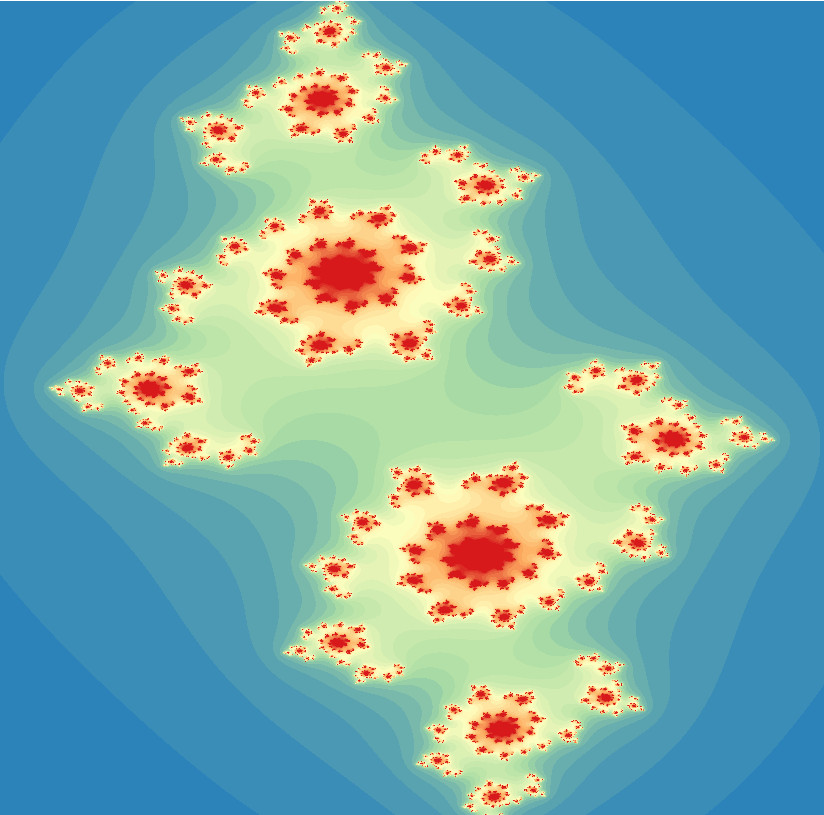
\includegraphics[scale=0.2]{./images/fractal16k16k}
\end{figure}
 
}

\frame{\frametitle{Julia Set - multi-GPU speedup} 
	\begin{figure}
	\centering
	\includegraphics[width=0.55\textwidth]{images/fractal_false_scaling}
	\caption{Julia set speedups obtained on single-GPU execution (K40 ,GTX980) and	multi-GPU execution on two devices ($144 \times 10^6$ grid points).}
\end{figure}
}

\frame{\frametitle{Julia Set - K40 vs GTX980} 
	\begin{figure}
		\centering
		\includegraphics[width=1\textwidth]{images/fractal12k_k40_980_true}
		\caption{Time and Speed-up for the Julia Set case ($1200 \times 10^6$ grid points) on two different GPUs: 1
			GTX980 and 1 K40 . The bottom and top horizontal axes indicate the amount of rows assigned to the K40 and GTX980 , respectively. .}
	\end{figure}
}


\subsection{Convolutional Filtering}
\frame{\frametitle{Convolutional Filtering} 
	\begin{itemize}
		\item Very common in image processing 
		\item The value of the grid point is substituted with a weighted average of neighboring points
		\item Little floating-point computation involved $\Longrightarrow$ memory bound
\end{itemize}
\begin{figure}
	\centering
	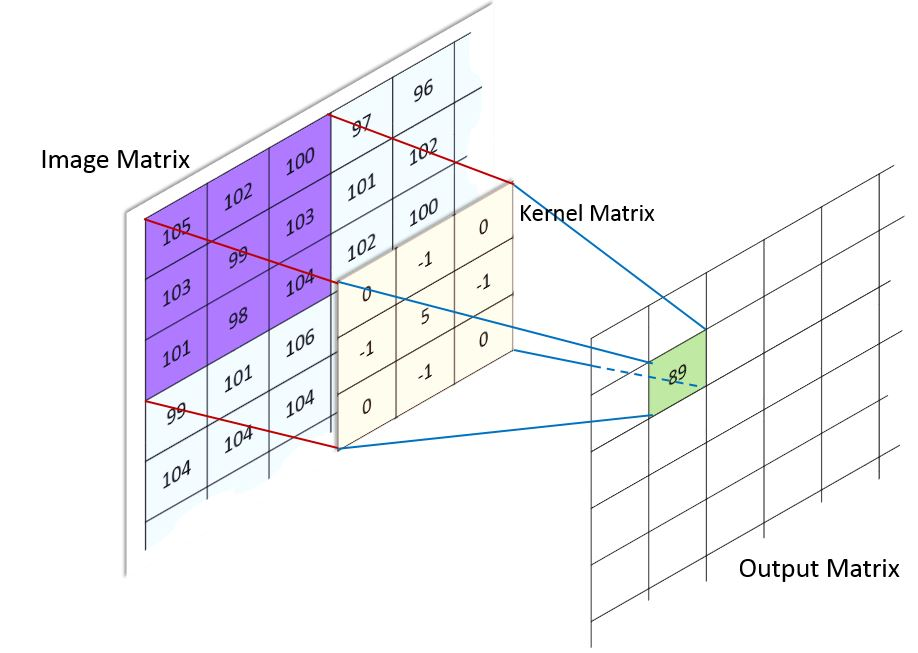
\includegraphics[scale=0.35]{./images/1}
\end{figure}

}







\end{document}

